%%%%%%%%%%%%%%%%%%%%%%%%%%%%%%%%%%%%%%%%%
% Vertical Line Title Page 
% LaTeX Template
% Version 1.0 (27/12/12)
%
% This template has been downloaded from:
% http://www.LaTeXTemplates.com
%
% Original author:
% Peter Wilson (herries.press@earthlink.net)
%
% License:
% CC BY-NC-SA 3.0 (http://creativecommons.org/licenses/by-nc-sa/3.0/)
% 
% Instructions for using this template:
% This title page compiles as is. If you wish to include this title page in 
% another document, you will need to copy everything before 
% \begin{document} into the preamble of your document. The title page is
% then included using \titleGM within your document.
%
%%%%%%%%%%%%%%%%%%%%%%%%%%%%%%%%%%%%%%%%%

%----------------------------------------------------------------------------------------
%	PACKAGES AND OTHER DOCUMENT CONFIGURATIONS
%----------------------------------------------------------------------------------------

\documentclass{book}

\usepackage{cite,graphicx}
\usepackage[chapter]{algorithm}
\usepackage{url,float}
\usepackage{hyperref}
\usepackage{uithesis}
\usepackage{listings}
\usepackage[nodayofweek,level]{datetime}
\usepackage[bahasai]{babel}
\usepackage{subfigure}
\usepackage{booktabs}
\selectlanguage{bahasai}
\newcommand*{\escape}[1]{\texttt{\textbackslash#1}}
\renewcommand{\bibname}{Daftar Referensi}
\renewcommand{\contentsname}{Daftar Isi}
\renewcommand{\listfigurename}{Daftar Gambar}
\renewcommand{\listtablename}{Daftar Tabel}
\renewcommand\lstlistingname{Program}
\renewcommand\lstlistlistingname{Daftar Program}
\renewcommand{\chaptername}{BAB}
\renewcommand{\figurename}{\bo{Gambar}}
\renewcommand{\tablename}{\bo{Tabel}}
\renewcommand{\arraystretch}{1.5}
\Var{\kataPengantar}{Kata Pengantar}
\include{hype.indonesia}

\lstset{
  basicstyle=\ttfamily,
  columns=fullflexible,
  frame=single,
  breaklines=true,
  postbreak=\mbox{\textcolor{red}{$\hookrightarrow$}\space},
}

%----------------------------------------------------------------------------------------
%	TITLE PAGE
%----------------------------------------------------------------------------------------

\newcommand*{\titleGM}{\begingroup % Create the command for including the title page in the document
\hbox{ % Horizontal box
\hspace*{0.2\textwidth} % Whitespace to the left of the title page
\rule{1pt}{\textheight} % Vertical line
\hspace*{0.05\textwidth} % Whitespace between the vertical line and title page text
\parbox[b]{0.75\textwidth}{ % Paragraph box which restricts text to less than the width of the page

{\noindent\Huge\bfseries Dasar Pemrograman\\ Python\\ pada Keilmuan Data}\\[2\baselineskip] % Title
%{\large \textit{Diktat kuliah}}\\[4\baselineskip] % Tagline or further description
{\large \textsc{Dr. Arya Adhyaksa Waskita}} % Author name

\vspace{0.5\textheight} % Whitespace between the title block and the publisher
%\begin{figure}[H]
%
\includegraphics[scale=.2]{pics/logo.png}
%\end{figure}
%STMIK Eresha - 2020
%Powered by \LaTex

{\noindent Disiapkan untuk Teknik Informatika UNPAM menggunakan \LaTeX}\\[\baselineskip] % Publisher and logo
}}
\endgroup}

%----------------------------------------------------------------------------------------
%	BLANK DOCUMENT
%----------------------------------------------------------------------------------------

\begin{document}

%\addChapter{\kataPengantar}


% Removes page numbers

\titleGM % This command includes the title page
\pagenumbering{roman}
\setcounter{page}{0}
\tableofcontents
\listoffigures
\listoftables
\addChapter{Daftar Program}
\lstlistoflistings
\addChapter{\kataPengantar}
%-----------------------------------------------------------------------------%
\chapter*{Kata Pengantar}
%-----------------------------------------------------------------------------%
Dengan berkembang pesatnya keilmuan data (\textit{data science}), mahasiswa dan dosen perlu menguasai \textit{tools} yang dapat menunjang aktifitas mereka untuk mengeksporasi keilmuan tersebut. Salah satu \textit{tools} yang umum digunakan dalam keilmuan data berbasis pemrograman python. Karena alasan tersebut, buku elektronik ini disusun.

Secara umum, diktat ini dibagi ke dalam bagian pendahuluan yang membahas tentang sejarah singkat Python yang dilanjutkan ke bagian instalasi. Instalasi ini, meskipun sangat sederhana, terutama pada sistem operasi Linux, dapat menjadi sangat merepotkan bagi beberapa mahasiswa, terutama ketika mereka menggunakan sistem operasi Windows. Karena itu, instalasi akan dilakukan di sistem operasi Windows. Bagian selanjutnya adalah dasar-dasar pemrograman Python, terutama struktur data (\texttt{list}, \texttt{tuple} dan \texttt{dictionary}), interaksi dengan \textit{file} dan basis data, hingga membuat modul yang dapat digunakan kembali. Akhirnya, selamat mencoba pengalaman baru. 

\vspace*{2cm}
\begin{flushright}
\selectlanguage{bahasai}
Serpong, \today\\[0.1cm]
\vspace*{1cm}
Dr. Arya Adhyaksa Waskita

\end{flushright}


\pagenumbering{arabic}
%\chapter{Sejarah Pemrograman Python}
\chapter{Pendahuluan}
\section{Sejarah singkat}
Python dibangun oleh Guido van Rossum (\figurename~\ref{fig:guido}\footnote{\url{https://gvanrossum.github.io/images/guido-headshot-2019.jpg}}) pada sekitar tahun 1980 di \textit{Centrum Wiskunde \& Informatica} (CWI) di Belanda\cite{python3intro}. Nama Python diambil dari program TV favorit Guido yang berjudul '''Monty Pythons Flying Circus''' yang tayang pada kisaran tahun 1969-1974.

\begin{figure}
  \begin{center}
    
\includegraphics[scale=.5]{pics/guido-headshot-2019.jpg}
    \caption{Guido van Rossum}
    \label{fig:guido}
  \end{center}
\end{figure}

\section{Kenapa Python?}
Berikut adalah beberapa jawaban dari pertanyaan tersebut.
\begin{itemize}
  \item \textit{Multiplatform}. Python adalah bahasa pemrograman yang tersedia pada sejumlah \textit{platform} sistem operasi seperti \texttt{GNU Linux, Windows dan Mac}. Selain itu, Python juga tersedia pada \textit{platform} perangkat bergerak seperti Android dan \textit{embedded system}\footnote{\url{https://wiki.python.org/moin/EmbeddedPython}}.
  \item Mudah. Python merupakan bahasa pemrograman yang mudah karena \texttt{syntax} yang sederhana, sehingga mudah dikuasai bahkan oleh pengguna yang tidak memiliki latar belakang pendidikan formal di bidang ilmu komputer.
  \item Pustaka. Pustaka pendukung untuk banyak bidang ilmu tersedia secara bebas (bahkan terawat dengan baik oleh komunitas), terutama dalam keilmuan data di mana Python sangat populer saat ini \footnote{\url{https://towardsdatascience.com/top-9-languages-for-data-science-in-2020-824239f930c}}. Setidaknya, hal itu disebabkan oleh pustaka Python yang tersedia untuk tujuan \textit{data collection and cleansing}, \textit{data exploration}, \textit{data modeling} dan \textit{data visualization and interpretation} \footnote{\url{https://www.kdnuggets.com/2020/01/python-preferred-languages-data-science.html}}.
\end{itemize}

\section{Keilmuan data}
Keilmuan data secara umum didefinisikan sebagai metodologi yang darinya, \textit{actionable insight} dapat disimpulkan dari data sebagai dasar dalam pengambilan keputusan\cite{igual2017introduction}. Keilmuan data sangat multidisiplin dengan basis keilmuan utama ada pada ilmu komputer, statistik, dan domain ilmu lain yang menjadi obyek kajian\cite{skiena2017data} seperti ilustrasi di \figurename~\ref{fig:wordcloud}. Selain sifatnya sebagai keilmuan multidisiplin yang menjembatani teori, komputasi, eksperimen, dan \textit{biosocial area}, keilmuan data juga memerlukan interaksi dengan data dengan ukuran sangat besar, dinamis dan tidak selaras (\textit{incongruent})\cite{dinov2018data}. Karena itu, diperlukan algoritma, metode, \textit{tools} dan layanan yang mampu mengolah data tersebut dan menghasilkan sistem pendukung keputusan yang semi otomatis.

\begin{figure}
  \begin{center}
    \includegraphics{pics/wordcloud4datascience.png}
    \caption{\textit{Word cloud} untuk saling keterkaitan dalam keilmuan data \cite{braschler2019applied}}
    \label{fig:wordcloud}
  \end{center}
\end{figure}

Algoritma dan metode yang diperlukan untuk menghasilkan sistem pendukung keputusan saat ini banyak memanfaatkan pembelajaran mesin dan kecerdasan buatan, selain statistik sebagai pondasi keilmuannya. \figurename~\ref{fig:piramida} menunjukkan piramida di mana ilmuan data berperan\footnote{\url{https://towardsdatascience.com/data-engineer-vs-data-scientist-bc8dab5ac124}} dalam hirarki yang pertama kali dibuat oleh Monica Rogati\footnote{\url{https://medium.com/hackernoon/the-ai-hierarchy-of-needs-18f111fcc007}}. Berdasarkan hirarki tersebut, pelatihan ini mengasumsikan bahwa data telah tersedia (terutama dalam format CSV). Selanjutnya, peserta harus mampu berinteraksi dengan data tersebut, terutama untuk tujuan praproses sebelum nantinya diolah dengan algoritma tertentu memanfaatkan pustaka berbasis Python.

\begin{figure}
  \begin{center}
    \includegraphics[scale=.5]{pics/piramida.png}
    \caption{Hirarki kebutuhan kecerdasan buatan}
    \label{fig:piramida}
  \end{center}
\end{figure}


\chapter{Instalasi Python}
\section{Interpreter Python}
\label{sec:interpreter}
Seperti telah dijelaskan di bagian Pengantar, instalasi \textit{interpreter} Python dilakukan di sistem operasi Windows 7. Tahapan instalasi ini mengasumsikan bahwa tidak ada kendala apapun terkait sistem operasi. Selanjutnya mahasiwa diminta untuk mengunduh \textit{interpreter} Python melalui laman \url{https://www.python.org/downloads/} sesuai kebutuhannya. 

Mengeksekusi unduhan tersebut akan memunculkan dialog seperti pada \figurename~\ref{fig:install1}. Pastikan untuk memilih konfigurasi \texttt{PATH} secara otomatis agar ketika proses instalasi selesai, \textit{interpreter} Python dapat dijalankan dari mana saja di sistem komputer masing-masing. Untuk kondisi di mana terjadi kesalahan, akan muncul dialog yang memberi kita kesempatan untuk melihat \textit{log}. Buka log tersebut dan lihat sumber dari kesalahan instalasi yang sedang terjadi.

\begin{figure}[h!]
   \begin{center}
     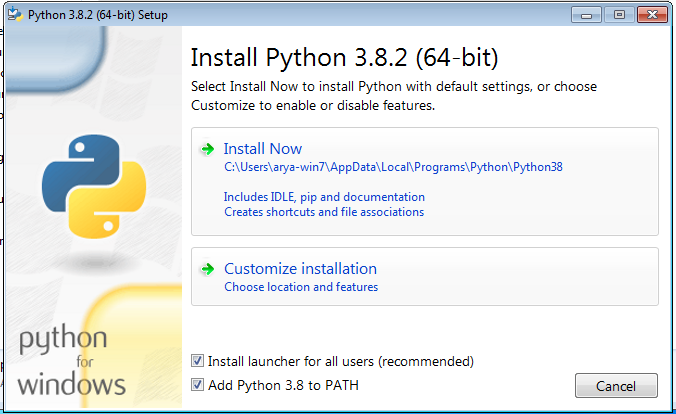
\includegraphics[scale=.5]{pics/installPython1.png}
     \caption{Dialog instalasi \textit{interpreter} Python}
     \label{fig:install1}
   \end{center}
 \end{figure} 

Pilihan opsi \textit{Customize installation} akan menampilkan dialog seperti \figurename~\ref{fig:feature}. Pastikan semua pilihan dipilih. Kemudian, selama proses instalasi berlangsung, pengguna akan disuguhkan dialog seperti \figurename~\ref{fig:installProgres}. Tunggu sampai dialog tanda selesai dikeluarkan seperti pada \figurename~\ref{fig:finish}.

\begin{figure}[h!]
  \begin{center}
    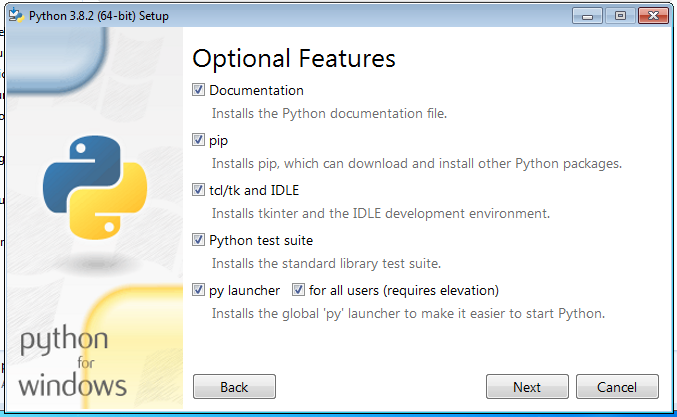
\includegraphics[scale=.5]{pics/featureInstall.png}
    \caption{Pilihan paket pendukung sebelum instalasi dilakukan}
    \label{fig:feature}
  \end{center}
\end{figure}

\begin{figure}[h!]
  \begin{center}
    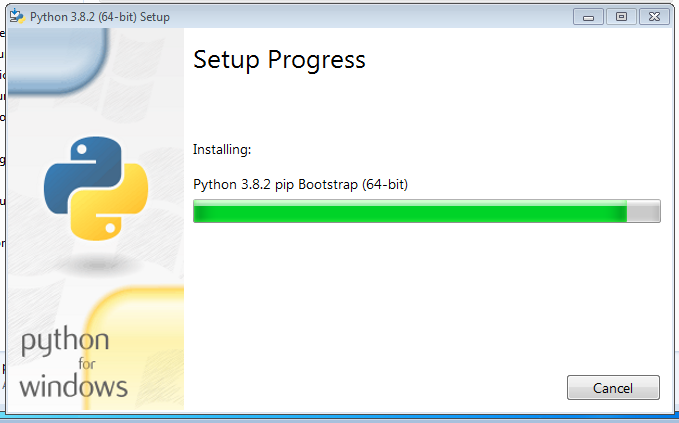
\includegraphics[scale=.5]{pics/installProgress.png}
    \caption{Dialos selama proses instalasi berlangsung}
    \label{fig:installProgres}
  \end{center}
\end{figure}

\begin{figure}[h!]
  \begin{center}
    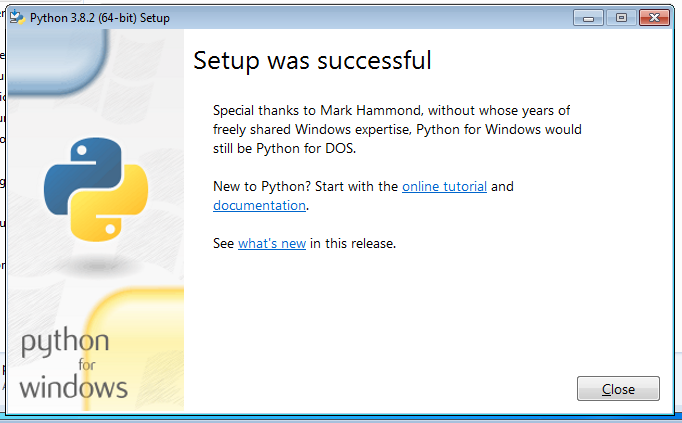
\includegraphics[scale=.5]{pics/installFinished.png}
    \caption{Dialog tanda selesai instalasi}
    \label{fig:finish}
  \end{center}
\end{figure}

Seperti telah ditunjukkan pada \figurename~\ref{fig:install1} tentang informasi lokasi \textit{interpreter} Python diletakkan, dapat juga dibuktikan melalui aplikasi \texttt{CMD} seperti \figurename~\ref{fig:lokasi}. Sedangkan \textit{interpreter} Python dapat diujicobakan dengan menuliskan perintah \texttt{python} di aplikasi \texttt{CMD}. Akan muncul dialog seperti \figurename~\ref{fig:siap}. \textit{Interpreter} Python siap digunakan, ditandai dengan munculnya karakter \texttt{>>>}.

\begin{figure}[h!]
  \begin{center}
    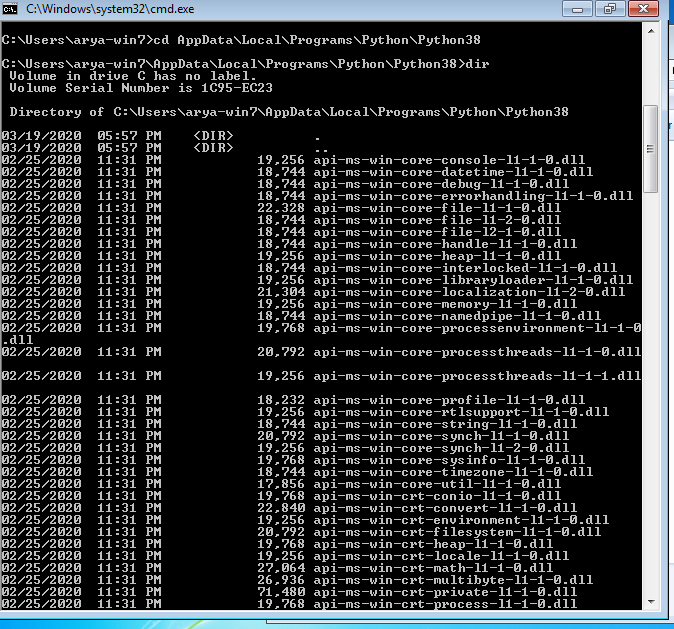
\includegraphics[scale=.5]{pics/installedLocation.png}
    \caption{Lokasi instalasi \textit{interpreter} Python}
    \label{fig:lokasi}
  \end{center}
\end{figure}

\begin{figure}[h!]
  \begin{center}
    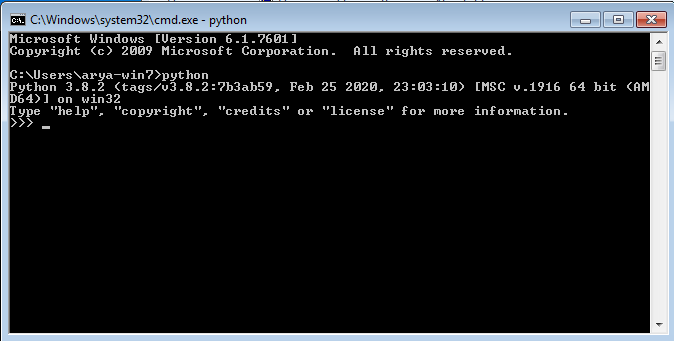
\includegraphics[scale=.5]{pics/pythonAktif.png}
    \caption{\textit{Interpreter} Python siap digunakan}
    \label{fig:siap}
  \end{center}
\end{figure}

Tahapan selanjutnya adalah instalasi pustaka \texttt{scikit-image}. Proses instalasinya dilakukan dengan aplikasi pengelola paket Python yang bernama \texttt{pip}. Silakan lihat \figurename~\ref{fig:feature}. \texttt{pip} ada di urutan kedua dari fitur tambahan. \texttt{pip} dapat digunakan untuk melihat paket apa saja yang telah terpasang di sistem kita. Caranya dengan menjalankan perintah \texttt{python -m pip list} seperti ditunjukkan \figurename~\ref{fig:daftarPaket}.

\begin{figure}[h!]
  \begin{center}
    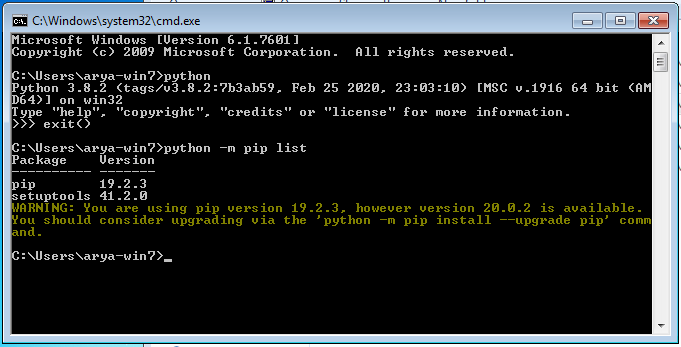
\includegraphics[scale=.5]{pics/pipList.png}
    \caption{Daftar paket yang terpasang}
    \label{fig:daftarPaket}
  \end{center}
\end{figure}

\texttt{pip} dapat juga digunakan untuk meng-\texttt{upgrade} paket yang telah terpasang, bahkan dirinya sendiri. Untuk meng-\textit{upgrade} paket \texttt{pip} itu sendiri, dapat dilakukan dengan menjalankan perintah \texttt{python -m pip install --upgrade pip} seperti \figurename~\ref{fig:pipUpgrade}. Perhatikan versi \texttt{pip} yang ada di \figurename~\ref{fig:daftarPaket} dan \figurename~\ref{fig:pipUpgrade}.
 
\begin{figure}
  \begin{center}
    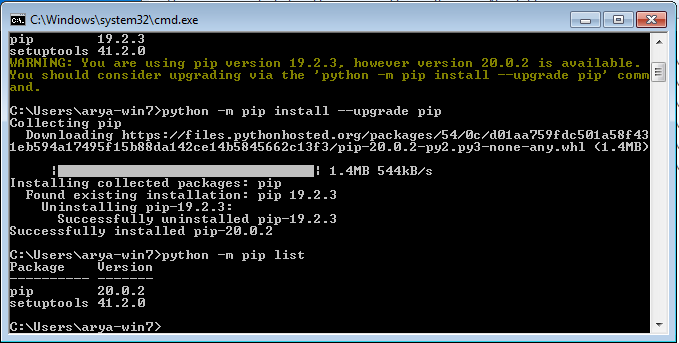
\includegraphics[scale=.5]{pics/pipList2.png}
    \caption{Hasil \texttt{upgrade} pip}
    \label{fig:pipUpgrade}
  \end{center}
\end{figure}


Setelah selesai, kita dapat kembali melihat daftar paket yang terpasang melalui pengelolaan \texttt{pip} yang ditunjukkan \figurename~\ref{fig:daftarPaket2}.

\begin{figure}[h!]
  \begin{center}
    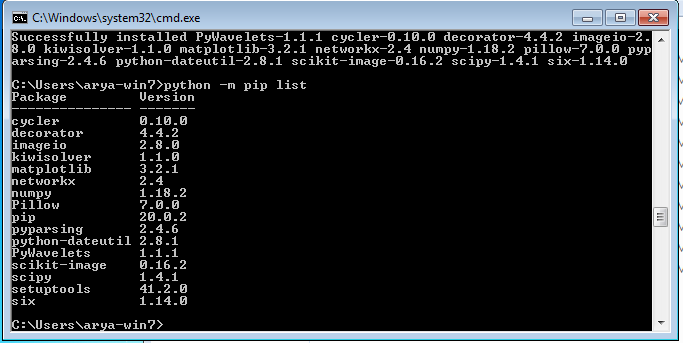
\includegraphics[scale=.5]{pics/pipList3.png}
    \caption{Daftar terakhir paket terpasang}
    \label{fig:daftarPaket2}
  \end{center}
\end{figure}

Menu aplikasi pendukung Python akan muncul seperti \figurename~\ref{fig:menu}. Menu kedua pada \figurename~\ref{fig:menu} akan memunculkan aplikasi \texttt{CMD} yang sama dengan yang ditunjukkan \figurename~\ref{fig:siap}, tetapi tanpa perlu memanggil perintah \texttt{python} terlebih dahulu. CMD secara otomatis akan memunculkan Python \texttt{shell} seperti \figurename~\ref{fig:siap}.

\begin{figure}[h!]
  \begin{center}
    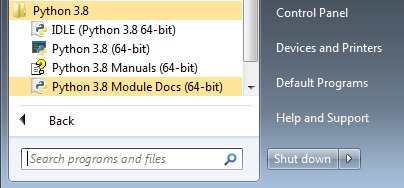
\includegraphics[scale=.5]{pics/menuPython.png}
    \caption{Daftar menu aplikasi pendukung Python}
    \label{fig:menu}
  \end{center}
\end{figure}

\texttt{IDLE} adalah antarmukan \textit{interpreter} Python seperti ditunjukkan \figurename~\ref{fig:idle}. Dalam \figurename~\ref{fig:idle} juga terlihat bahwa kita berhasil meng-\textit{import} pustaka \texttt{scikit-image}, yang dalam \texttt{IDLE} di Windows 7 disebut sebagai \texttt{skimage}. Jika Anda sedang menggunakan Ubuntu, kemudian menggunakan pustaka \texttt{scikit-image} yang diperoleh dari \textit{repository} Ubuntu (bukan dari \texttt{pip}), pustaka \texttt{scikit-image} juga di-\textit{import} dengan nama \texttt{skimage}. Berhasilnya sebuah pustaka Python di-\textit{import} adalah ketika tidak ada komentar yang muncul setelah perintah \texttt{import} tersebut.

\begin{figure}
  \begin{center}
    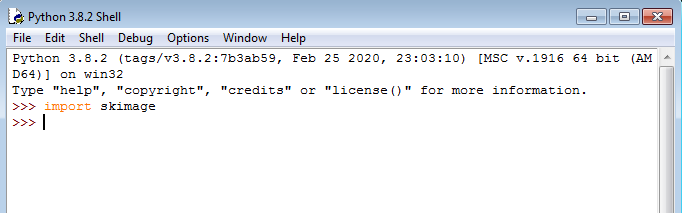
\includegraphics[scale=.5]{pics/idle.png}
    \caption{Aplikasi \texttt{IDLE}}
    \label{fig:idle}
  \end{center}
\end{figure}

Selanjutnya, jika ditemukan petunjuk untuk masuk ke Python \texttt{Shell}, Anda dapat menggunakan aplikasi \texttt{IDLE}\texttt{}, atau menggunakan terminal (di Linux)/\texttt{CMD} (di Windows) dengan terlebih dahulu menjalankan perintah \texttt{python}.

\section{Anaconda}
Selain pilihan manual seperti yang telah dijelaskan di Sub bab \ref{sec:interpreter}, Anaconda bisa menjadi opsi lain yang lebih bersifat otomatis. Saya menyebutnya otomatis karena Anaconda sejumlah pustaka Python, terutama yang banyak digunakan di \textit{Data Mining}, \textit{Machine Learning} atau \textit{Data Science} telah dikemas di dalam Anaconda. Bahkan beberapa editor yang populer untuk Python juga dikemasnya. Anaconda bahkan mengemasnya khusus untuk \textit{platform} yang berbeda. Anda dapat menghubungi alamat \url{https://www.anaconda.com/} untuk mengunduh aplikasinya. Sesuaikan kebutuhan Anda dengan pilihan yang ada seperti ditunjukkan \figurename~\ref{fig:platformAnaconda}.

\begin{figure}
  \begin{center}
    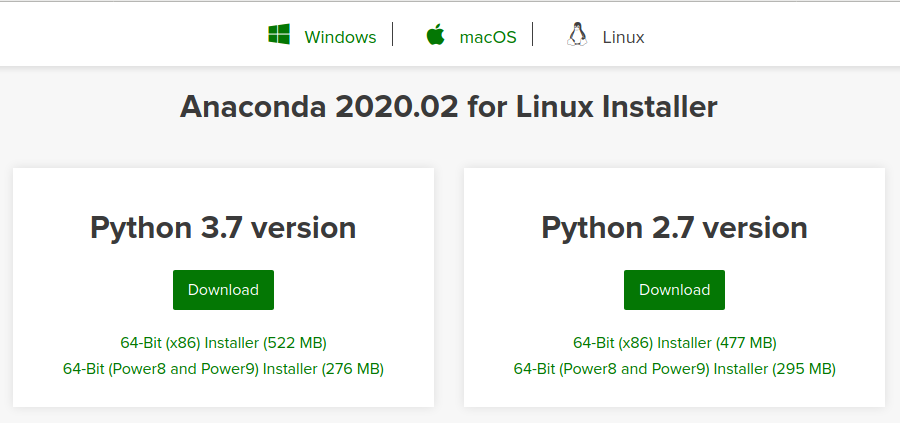
\includegraphics[scale=.5]{pics/anacondaInstall0.png}
    \caption{Pilihan \textit{platform} instalasi Anaconda}
    \label{fig:platformAnaconda}
  \end{center}
\end{figure}

Instalasi Anaconda akan menghadirkan dialog seperti ditunjukkan \figurename~\ref{fig:pembuka} - \figurename~\ref{fig:instalasiEnd}. Anaconda akan meletakkan pustaka di lokasi \texttt{C:\textbackslash\textbackslash ProgramData\textbackslash\textbackslash Anaconda3} yang berbeda dengan \texttt{pip} seperti terlihat di \figurename~\ref{fig:target}. Sedangkan di \figurename~\ref{fig:prosesInstalasi} terlihat sejumlah pustaka penting seperti \texttt{scikit-image} dan \texttt{scikit-learn} tengah diinstal. 

\begin{figure}aplikasi ini akan menghadirkan antarmuka seperti tampak
  \begin{center}
    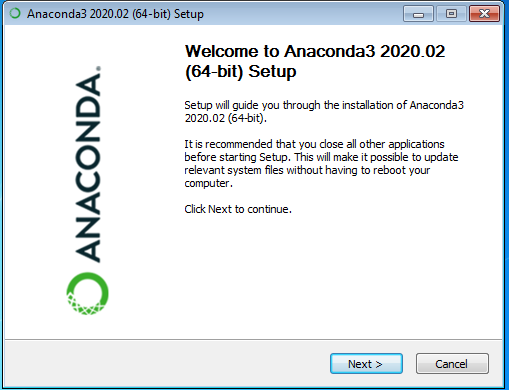
\includegraphics[scale=.5]{pics/anacondaInstall1.png}
    \caption{Dialog pembuka instalasi}
    \label{fig:pembuka}
  \end{center}
\end{figure}

\begin{figure}
  \begin{center}
    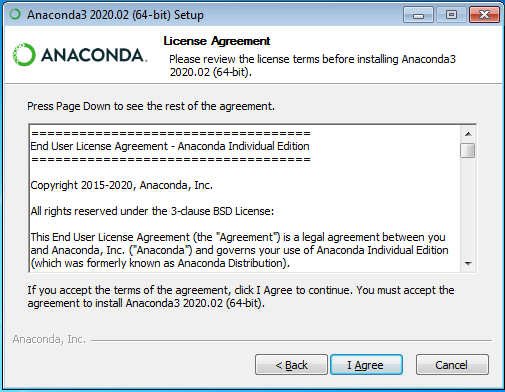
\includegraphics[scale=.5]{pics/anacondaInstall2.png}
    \caption{Menyetujui kesepakatan}
    \label{fig:kesepakatan}
  \end{center}
\end{figure}

\begin{figure}
  \begin{center}
    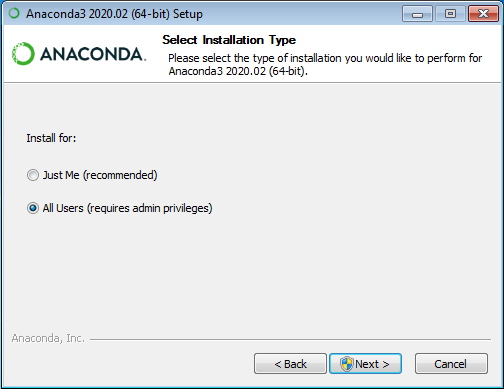
\includegraphics[scale=.5]{pics/anacondaInstall3.png}
    \caption{Pilihan pengguna Anaconda}
    \label{fig:pengguna}
  \end{center}
\end{figure}

\begin{figure}
  \begin{center}
    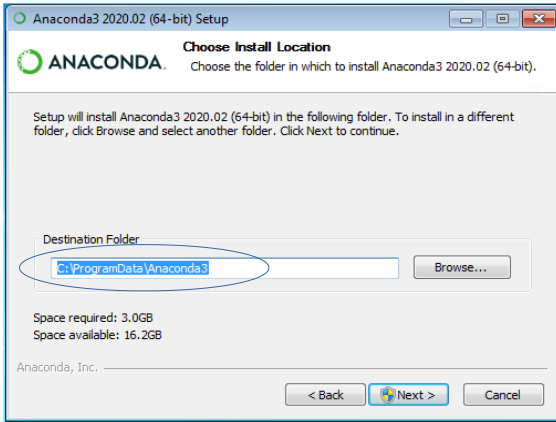
\includegraphics[scale=.5]{pics/anacondaInstall4a.png}
    \caption{Target instalasi}
    \label{fig:target}
  \end{center}
\end{figure}

\begin{figure}
  \begin{center}
    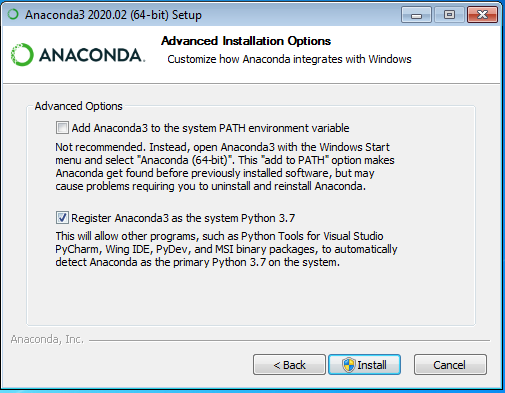
\includegraphics[scale=.5]{pics/anacondaInstall5.png}
    \caption{Menjadikan Anaconda sebagai sistem utama Python}
    \label{fig:utama}
  \end{center}
\end{figure}

\begin{figure}
  \begin{center}
    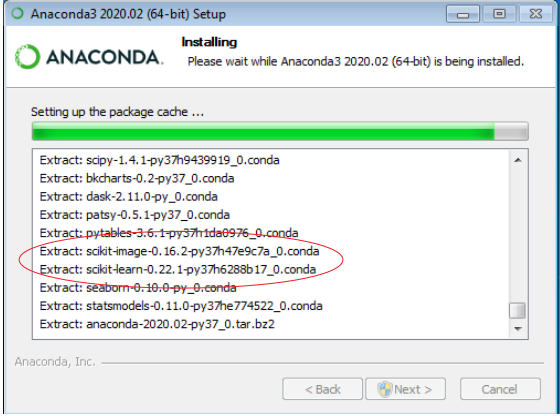
\includegraphics[scale=.5]{pics/anacondaInstall6a.png}
    \caption{Proses instalasi}
    \label{fig:prosesInstalasi}
  \end{center}
\end{figure}

\begin{figure}
  \begin{center}
    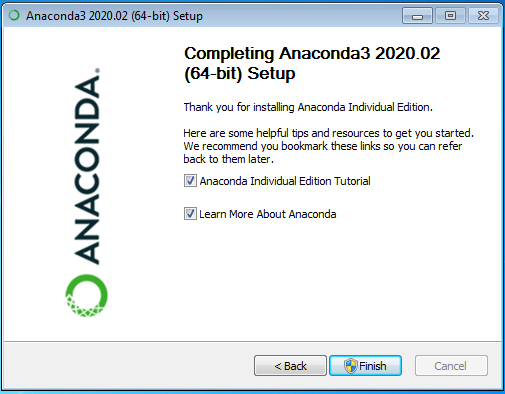
\includegraphics[scale=.5]{pics/anacondaInstall9.png}
    \caption{Instalasi selesai}
    \label{fig:instalasiEnd}
  \end{center}
\end{figure}

Instalasi Anaconda akan membuat menu seperti pada \figurename~\ref{fig:menuAnaconda}. Di situ terlihat sejumlah aplikasi yang dapat digunakan untuk mengembangkan kode komputer berbasis Python seperti Jupyter dan Spyder. Untuk Jupyter, aplikasi ini akan menghadirkan antarmuka seperti tampak pada \figurename~\ref{fig:jupyter}. Di sisi kanan atas terlihat beberapa opsi antarmuka untuk mengelola proyek Python dengan Jupyter, seperti Terminal \figurename~\ref{fig:jupyterTerminal} atau Python \texttt{Shell} di bawah Jupyter seperti \figurename~\ref{fig:jupyterShell} yang perannya seperti \texttt{IDLE} di \figurename~\ref{fig:idle}. Sedangkan untuk Spyder, akan tampak antarmuka seperti \figurename~\ref{fig:spyder}.

\begin{figure}
  \begin{center}
    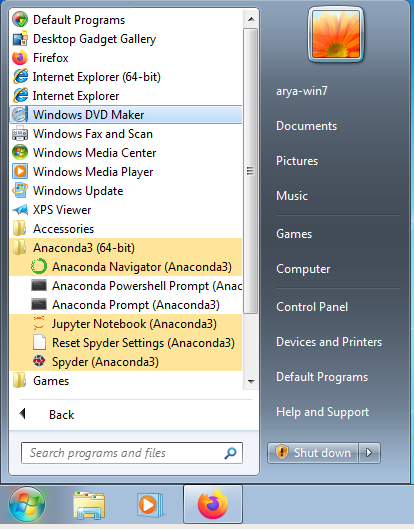
\includegraphics[scale=.5]{pics/anacondaMenu2.png}
    \caption{Anaconda yang tampil di Menu Ms. Windows$\copyright$}
    \label{fig:menuAnaconda}
  \end{center}
\end{figure}

\begin{figure}
  \begin{center}
    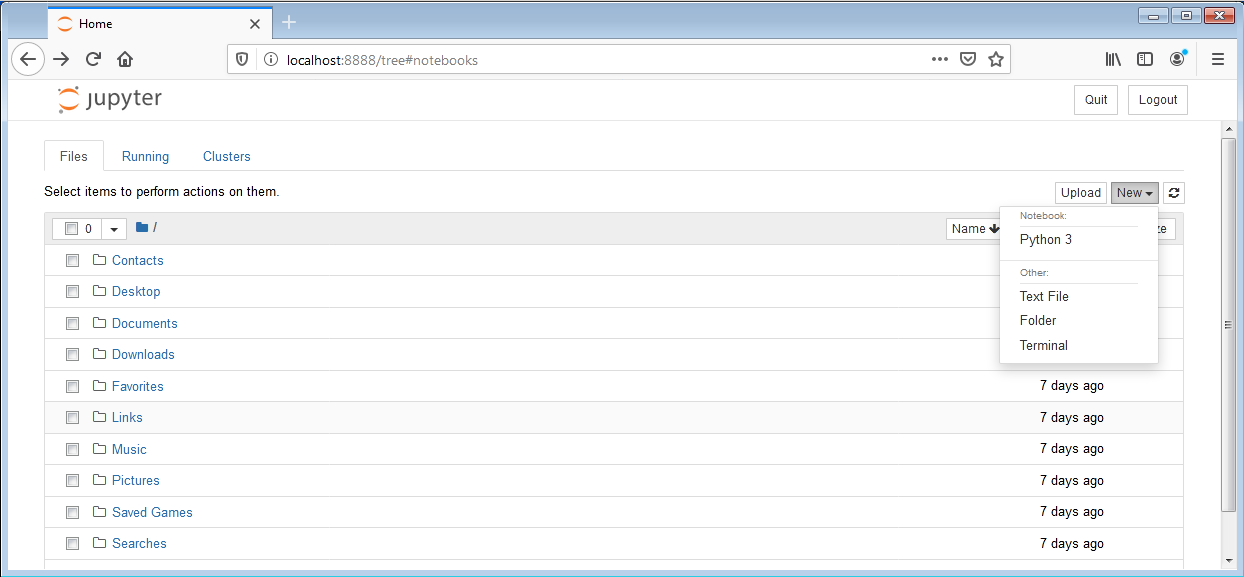
\includegraphics[scale=.5]{pics/jupyter2.png}
    \caption{Aplikasi \texttt{Jupyter}}
    \label{fig:jupyter}
  \end{center}
\end{figure}

\begin{figure}
  \begin{center}
    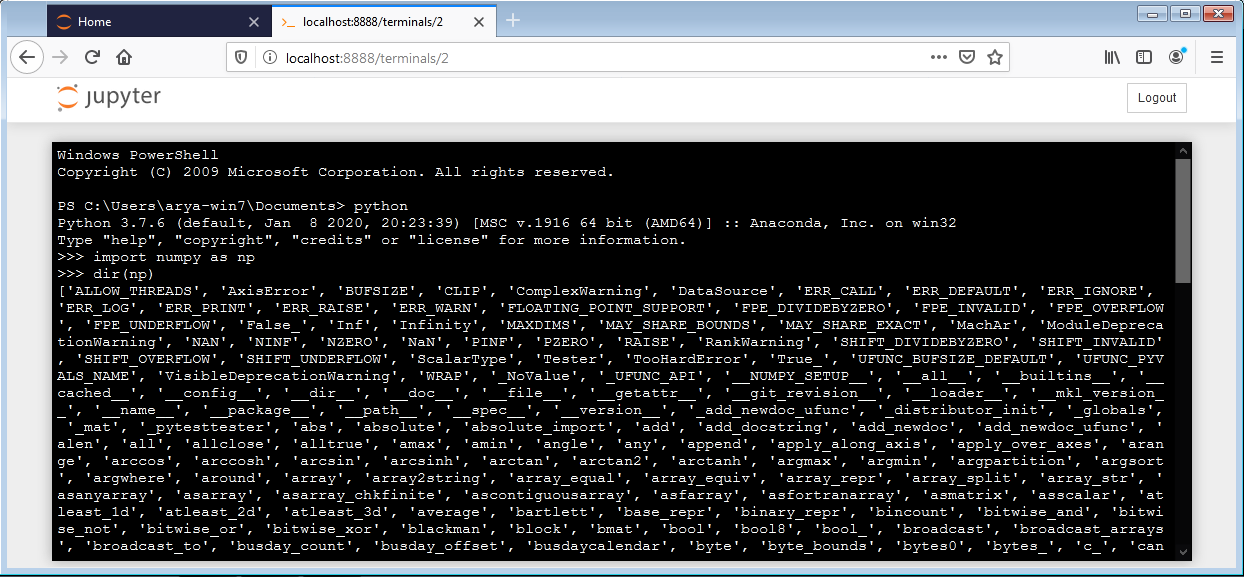
\includegraphics[scale=.5]{pics/jupyter3.png}
    \caption{Terminal pada aplikasi \texttt{Jupyter}}
    \label{fig:jupyterTerminal}
  \end{center}
\end{figure}

\begin{figure}
  \begin{center}
    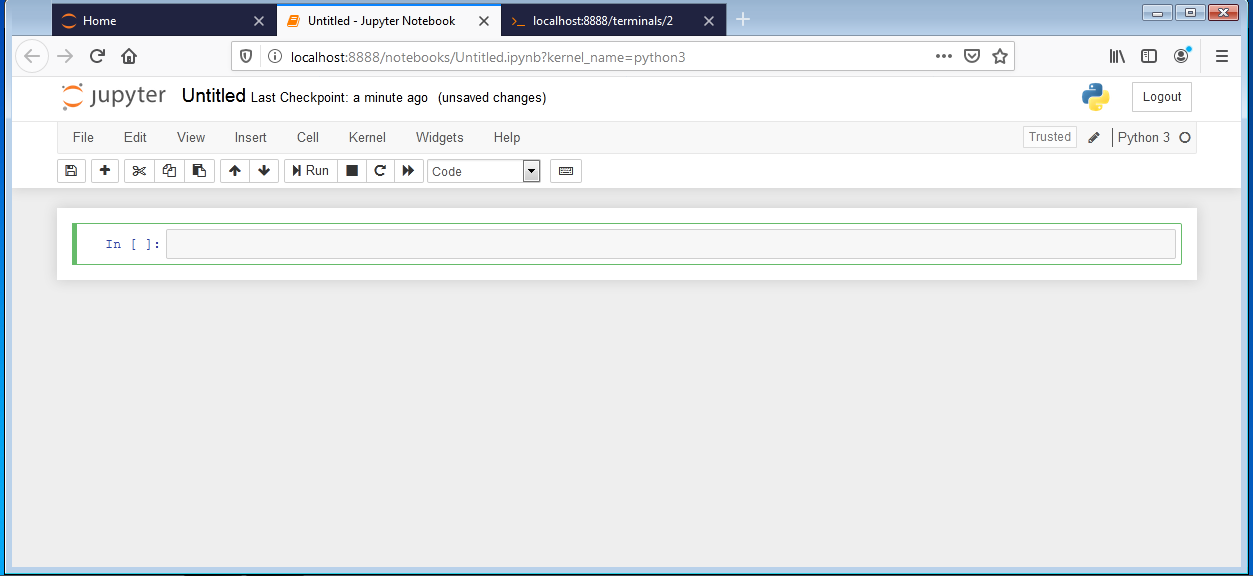
\includegraphics[scale=.5]{pics/jupyter4.png}
    \caption{Python \texttt{Shell} pada aplikasi \texttt{Jupyter}}
    \label{fig:jupyterShell}
  \end{center}
\end{figure}

\begin{figure}
  \begin{center}
    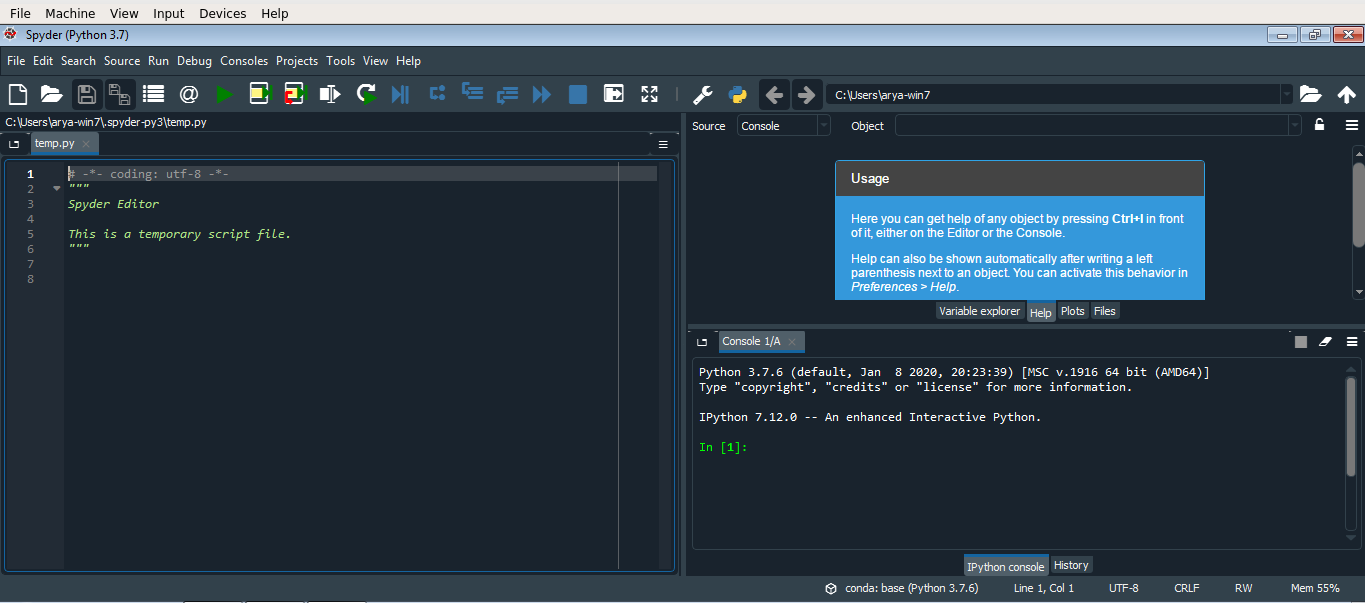
\includegraphics[scale=.45]{pics/spyder.png}
    \caption{Aplikasi \texttt{Spyder}}
    \label{fig:spyder}
  \end{center}
\end{figure}

\include{helloWorld}
\chapter{Dasar Pemrograman Python}
\section{Pendahuluan}
Bahasa pemrograman Python memiliki 4 sifat dasar berikut\footnote{\url{https://www.tutorialspoint.com/python/index.htm}}.
\begin{enumerate}
  \item \textit{Interpreter}. Python diproses oleh \textit{interpreter}, sehingga tidak perlu dikompilasi untuk menjalankannya. Hal ini seperti dijumpai pada bahasa pemrograman PHP yang sangat populer itu.
  \item Interaktif. Anda dapat berinteraksi denga Python dengan memberikannya perintah satu per satu melalui Python \texttt{shell}. Setiap perintah yang diberikan langsung akan direspon. Selain itu, Python bersifat \textit{self explained}. Jika ada fungsi dari suatu obyek yang tidak kita ketahui, kita bisa mempelajarinya langsung dari dokumentasi di Python \texttt{shell}.
  \item Berorientasi obyek. Ada semacam slogan bahwa '''\textit{Everything is object in Python}'''. Seperti telah dipahami melalu kuliah Rekayasa Perangkat Lunak, orientasi obyek menyebabkan variabel dan fungsi (sering disebut sebagai \textit{state} dan \textit{behavior}) terkemas dalam sebuah obyek, sehingga memudahkan pengelolaan variabel. Fungsi yang melekat pada sebuah obyek juga dapat diturunkan dari satu obyek ke obyek lain sehingga tidak perlu dideklarasi ulang. Namun, fitur orientasi obyek ini pemberlakuannya bagi pemrogram tidak seketat seperti yang dilakukan di \texttt{Java}. Jika \texttt{Java} mengharuskan pemrogram mendeklarasikan kelas untuk membuat program yang bahkan sangat sederhana, maka Python tidak mengharuskannya.
  \item Bahasa pemrograman untuk pemula. Hal ini disebabkan karena Python sangat sederhana, tidak memerlukan banyak deklarasi yang seringkali menyulitkan, bahkan menakutkan bagi pemula. Selain itu, Python juga mendukung pengembangan aplikasi untuk banyak \textit{platform}, dari aplikasi \textit{embedded} hingga \textit{web} dan \textit{mobile}. 
\end{enumerate}

Untuk sifat dasar pertama dan kedua, dapat dilihat ilustrasinya di \figurename~\ref{fig:interpreter}. Dalam \figurename~\ref{fig:interpreter}, Python \texttt{shell} dipanggil dengan perintah \texttt{python3}. Hal tersebut disebabkan karena Ubuntu (yang sedang digunakan adalah Ubuntu 18.04) secara \textit{default} menyertakan Python versi 2.x. Sedangkan untuk Python versi 3.x harus dijalankan dengan perintah \texttt{python3}. Di \figurename~\ref{fig:interpreter} terlihat bahwa ada dua perintah yang diberikan secara berurutan. Tetapi, Python akan meresponnya satu per satu. Sedangkan untuk keluar dari Python \texttt{shell}, berikan perintah \texttt{exit()}.

\begin{figure}[h!]
  \begin{center}
    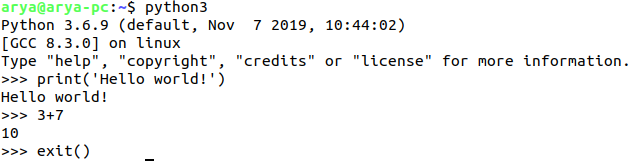
\includegraphics[scale=.5]{pics/interpreter.png}
    \caption{Python \texttt{shell} sedang menerima perintah}
    \label{fig:interpreter}
  \end{center}
\end{figure}

Untuk sifat dasar ketiga dapat diilustrasikan melalui \figurename~\ref{fig:obyek}. Kita dapat mengetahui jenis obyek dari variabel \texttt{a} dengan fungsi \texttt{type(a)}. Sedangkan untuk melihat fungsi dan variabel apa saja yang terkandung pada variabel \texttt{a}, kita dapat menggunakan fungsi \texttt{dir(a)}. Tetapi, meskipun semuanya di dalam Python adalah obyek, penggunaan Python tidak mengharuskan kita mendeklarasi kelas secara eksplisit. Dengan menuliskan perintah \texttt{a=3}, Python tahu bahwa obyek \texttt{a} adalah obyek dari kelas \texttt{integer}. Bahkan, di \figurename~\ref{fig:interpreter}, operasi aritmatika dapat dilakukan tanpa mendeklrasi variabel.

\begin{figure}[h!]
  \begin{center}
    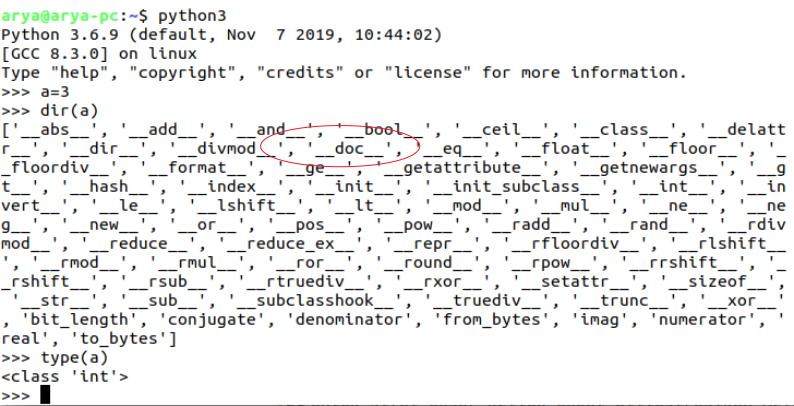
\includegraphics[scale=.5]{pics/interpreter2a.png}
    \caption{Variabel \texttt{a} sebagai obyek}
    \label{fig:obyek}
  \end{center}
\end{figure}

Di \figurename~\ref{fig:obyek} terlihat ada entitas yang diawali dan/atau diakhir dengan karakter dua \textit{underscore} ('\_\_') atau sering disebut sebagi \textit{dunder}\footnote{\url{https://dbader.org/blog/meaning-of-underscores-in-python}} (\textit{double undescore}) oleh komunitas pemrogram Python. Hal tersebut merupakan bagian dari PEP (\textit{Python Enhancement Proposals}) ke-8 tentang \textit{Style Guide for Python Code}\footnote{\url{https://www.python.org/dev/peps/pep-0008/}}.

Di \figurename~\ref{fig:obyek} juga terlihat bahwa obyek \texttt{a} memiliki fungsi \texttt{\_\_doc\_\_}. Fungsi inilah yang akan memberikan penjelasan singkat kepada kita tentang obyek yang sedang menjadi perhatian. Untuk menggunakannya, jalankan perintah \texttt{a.\_\_doc\_\_} seperti ditunjukkan \figurename~\ref{fig:doc}. Dengan \texttt{a} adalah nama variabel untuk obyek yang sedang menjadi perhatian.

\begin{figure}[h!]
  \begin{center}
    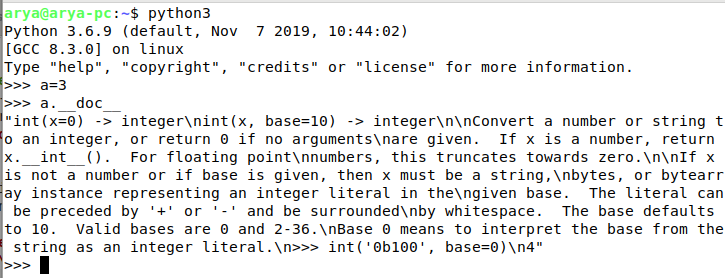
\includegraphics[scale=.5]{pics/interpreter3.png}
    \caption{Menampilkan dokumentasi obyek \texttt{integer a}}
    \label{fig:doc}
  \end{center}
\end{figure}

Format dokumentasi seperti yang ditunjukkan pada \figurename~\ref{fig:doc} sulit untuk dipahami. Pendekatan lain untuk mempelajari dokumentasi sebuah pustaka adalah dengan menggunakan fungsi \texttt{help}. Untuk kasus seperti \figurename~\ref{fig:doc}, perintah yang dijalankan adalah \texttt{help(a)} (\textbf{BUKAN} \texttt{a.\_\_doc\_\_}). Hasilnya ditunjukkan pada \figurename~\ref{fig:doc2}. Untuk keluar dari modus dokumentasi tersebut, pengguna tinggal memberi perintah \texttt{q} setelah tanda titik dua (\figurename~\ref{fig:doc2}). Sedangkan untuk melihat isi dokumentasi selanjutnya pengguna dapat menggunkana tombol spasi di papan ketik.

\begin{figure}
  \begin{center}
    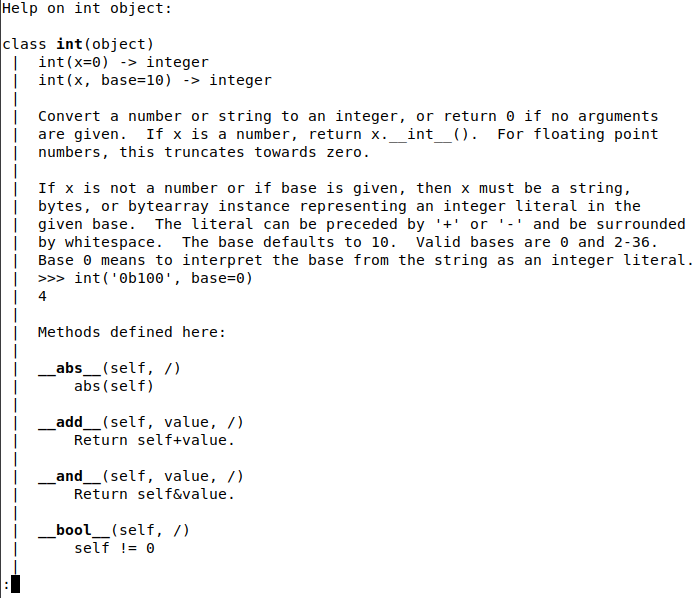
\includegraphics[scale=.5]{pics/interpreter4.png}
    \caption{Menampilkan dokumentasi obyek \texttt{integer a} menggunakan fungsi \texttt{help}}
    \label{fig:doc2}
  \end{center}
\end{figure}

\section{Struktur Data}
%http://thomas-cokelaer.info/tutorials/python/data_structures.html
Strukur data yang dimaksud di sini adalah data \textit{array}/larik dan sejenisnya, serta cara penggunaannya. Tidak jarang, fungsi dalam pustaka \textit{scikit-image} menerima argumen atau mengembalikan nilai dalam bentuk data \textit{array} atau sejenisnya. 
\subsection{\texttt{List}}
\textit{List} adalah \textit{array} yang paling banyak digunakan. Kita dapat menyimpan sejumlah nilai, dari tipe apapun ke dalam \texttt{list}, bahkan menambah atau mengurangi isinya. Untuk yang pernah mempelajari bahasa pemrograman C, tentu paham betapa sulitnya melakukan hal tersebut di C. Untuk C++ \texttt{list} dapat terapkan lebih mudah dengan bantuan \textit{standard template library}\footnote{\url{https://en.wikipedia.org/wiki/Standard\_Template\_Library}}

Sebuah variabel \texttt{list}, misalnya \texttt{a}, diinisiasi dengan perintah \texttt{a=[]}. Maka, variabel \texttt{a} memiliki sejumlah fungsi yang bisa dilihat dengan perintah \texttt{dir(a)}. Diktat ini hanya akan membahas fungsi-fungsi yang sering digunakan saja. Fungsi lain bisa dipelajari sendiri dengan bantuan perintah \texttt{help(a.nama\_fungsi)}, dengan \texttt{a} adalah obyek \texttt{list}.

\begin{enumerate}
  \item \texttt{append}. Fungsi ini menambahkan elemen baru ke variabel \texttt{list}. Perhatikan \figurename~\ref{fig:append}. Variabel \texttt{a} yang awalnya kosong, kemudian diisi satu per satu menggunakan perintah \texttt{append}. Variabel \texttt{a} terakhir memiliki dua elemen, masing-masing bertipe \texttt{integer} dan \texttt{character}.
  \begin{figure}
    \begin{center}
      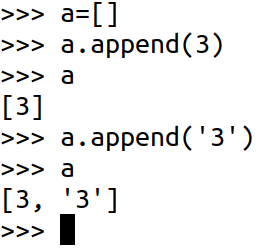
\includegraphics[scale=1.25]{pics/append.png}
      \caption{Proses penambahan elemen \texttt{list}}
      \label{fig:append}
    \end{center}
  \end{figure}
  
  \item \texttt{extend}. Fungsi ini memiliki tugas yang sama dengan \texttt{append} dengan sedikit perbedaan. Perhatikan \figurename~\ref{fig:extend}. Di \figurename~\ref{fig:extend1}, variabel \texttt{a} ditambahkan sebuah elemen berupa variabel list \texttt{b} menggunakan fungsi \texttt{append}. Variabel \texttt{b} yang telah memiliki dua elemen ditambahkan ke variabel \texttt{a} sebagai satu elemen. Hal tersebut terlihat dari dijalankannya perintah \texttt{len(a)}.
  
Sementara di \figurename~\ref{fig:extend2}, proses yang sama dilakukan menggunakan fungsi \texttt{extend}. Fungsi \texttt{extend} akan menambahkan variabel \texttt{b} ke dalam variabel \texttt{a} tidak sebagai \texttt{list} secara keseluruhan, tetapi menambahkan masing-masing elemen variabel \texttt{b} ke dalam \texttt{a}. Itu sebabnya, hasil penambahan \texttt{b} ke dalam \texttt{a} membuat \texttt{a} saat ini memiliki dua elemen.
  
\begin{figure}[h!]
\begin{center}
\subfigure[]{\label{fig:extend1}}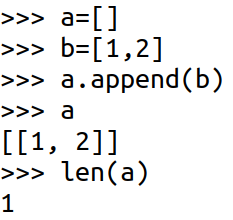
\includegraphics[scale=1.25]{pics/extend1.png}
\subfigure[]{\label{fig:extend2}}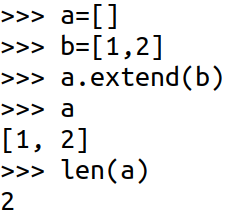
\includegraphics[scale=1.25]{pics/extend2.png}
\caption{Perbandingan penambahan elemen \texttt{list} menggunakan fungsi (a). \texttt{append} dan (b). \texttt{extend}}
\label{fig:extend}
\end{center}
\end{figure}

\item \texttt{insert}. Selain menambahkan elemen ke variabel \texttt{list} di posisi akhir, penambahan elemen juga dapat dilakukan di posisi tertentu. Perhatikan \figurename~\ref{fig:insert}. Penambahan karakter \texttt{'x'} pada posisi pertama dari \texttt{list} dilakukan dengan perintah \texttt{a.insert(0,'x')}. Hal ini disebabkan karena indeks dari elemen \texttt{list} dimulai dari \texttt{0}. 

\begin{figure}[h!]
  \begin{center}
    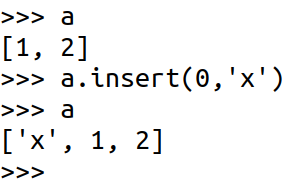
\includegraphics[scale=1.25]{pics/insert.png}
    \caption{Penambahan karakter 'x' ke variabel \texttt{a} di posisi pertama}
    \label{fig:insert}
  \end{center}
\end{figure}

\item \texttt{remove}. Selain menambahkan elemen ke variabel \texttt{list}, kita dapat juga membuang salah satu elemen yang ada di posisi tertentu di dalam \texttt{list}. Perhatikan figurename~\ref{fig:remove}. Perintah \texttt{remove} digunakan untuk mengeluarkan elemen tertentu dari \texttt{list}. Jika ada lebih dari satu elemen yang sama yang akan dikeluarkan, maka elemen terpilih untuk dikeluarkan adalah elemen yang muncul pertama kali pada \texttt{list}.

\begin{figure}[h!]
  \begin{center}
    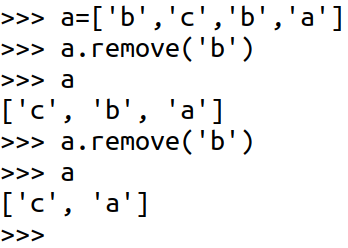
\includegraphics[scale=1.25]{pics/remove.png}
    \caption{Mengeluarkan elemen tertentu dari \texttt{list}}
    \label{fig:remove}
  \end{center}
\end{figure}

\item \texttt{pop}. Fungsi ini akan mengeluarkan elemen terakhir dari \texttt{list}. Perhatikan \figurename~\ref{fig:pop}.

\begin{figure}[h!]
  \begin{center}
    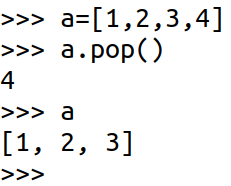
\includegraphics[scale=1.25]{pics/pop.png}
    \caption{Mengeluarkan elemen terakhir dari variabel \texttt{list}}
    \label{fig:pop}
  \end{center}
\end{figure}

\end{enumerate}
\subsection{\texttt{Tuple}}
\texttt{Tuple} adalah jenis \textit{array} selain \texttt{list} yang di Python dideklarasikan dengan perintah \texttt{a=()}. Operasi pada \texttt{tuple} lebih cepat dilakukan jika dibandingkan dengan \texttt{list}. Hal ini disebabkan karena \texttt{tuple} bersifat statis karena elemen yang ada di dalamnya tidak dapat diubah, kecuali yang bersifat \textit{mutable}. Karena bersifat statis, deklarasi variabel \texttt{a=()} tidak akan bermanfaat. Perhatikan \figurename~\ref{fig:tuple}.

Di \figurename~\ref{fig:tuple}, sebuah variabel \texttt{a} memiliki empat elemen, di mana elemen ke-4 merupakan sebuah \texttt{list}. Elemen ke-4 diakses dengan indeks \texttt{3} (karena indeks \texttt{tuple} dimulai dari \texttt{0}). Ketika diakes, isi dari elemen ke-4 tersebut dapat diubah karena bersifat \textit{mutable}. Sebaliknya, ketika elemen lain (dalam hal ini elemen ke-2) akan diubah nilainya, Python menolaknya. 

\begin{figure}[h!]
  \begin{center}
    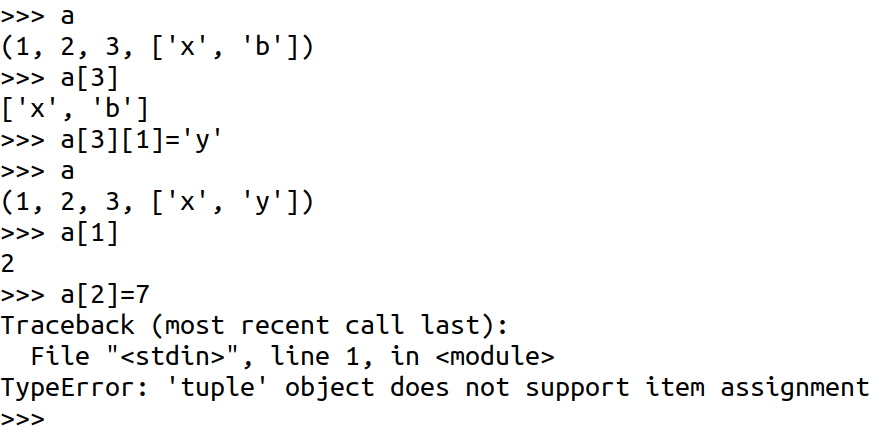
\includegraphics{pics/tuple.png}
    \caption{Beberapa operasi yang dilakukan pada variabel \texttt{tuple}}
    \label{fig:tuple}
  \end{center}
\end{figure}
 
\subsection{\texttt{Dictionary}}
\texttt{Dictionary} merupakan \textit{array} yang elemen penyusunnya merupakan pasangan \textit{key-value}. Setiap elemen akan diindeks berdasarkan \textit{key}. \texttt{Dictionary} dideklarasikan menggunakan perintah \texttt{a=\{\}}. Untuk menambah elemen ke variabel \texttt{dictionary}, gunakan perintah seperti \figurename~\ref{fig:dict}.

\begin{figure}[h!]
  \begin{center}
    
\includegraphics[scale=1.25]{pics/dictionary.png}
    \caption{Menambahkan elemen ke variabel \texttt{dictionary}}
    \label{fig:dict}
  \end{center}
\end{figure}

Kita juga dapat mengeluarkan sebuah elemen dari variabel \texttt{dictionary}. Karena elemennya merupakan pasangan \textit{key-value}, maka ketika dikeluarkan, pasangan \textit{key-value} tersebut tidak ada lagi di variabel \texttt{dictionary}. Perhatikan \figurename~\ref{fig:popDict}, elemen yang memiliki \textit{key} berupa karakter \texttt{'nama'} akan dikeluarkan menggunakan fungsi \texttt{pop}. Karena memerlukan argumen berupa \textit{key}, maka fungsi \texttt{pop} dapat mengeluarkan elemen yang posisinya di mana saja di dalam variabel \texttt{dictionary}, tidak harus di posisi terakhir.  

\begin{figure}
  \begin{center}
    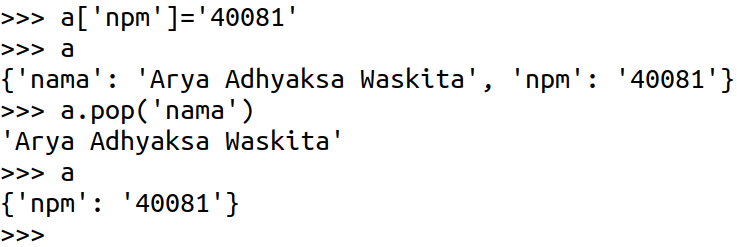
\includegraphics[scale=1.25]{pics/popDict.png}
    \caption{Mengeluarkan pasangan \textit{key-value} dari variabel \texttt{dictionary}}
    \label{fig:popDict}
  \end{center}
\end{figure}

\section{Operator}
\subsection{Aritmatika}
\tablename~\ref{tab:aritmatika} berisi operator aritmatika yang dimiliki Python\footnote{\url{https://www.w3schools.com/python/python_operators.asp}}. Untuk menggunakannya, variabel \texttt{a} dan \texttt{b} pada \tablename~\ref{tab:aritmatika} harus berjenis yang sama. Perhatikan \figurename~\ref{fig:aritmatika}. Tentunya, operasi seperti itu hanya berlaku untuk operator penjumlahan karena karakter memang tidak dapat menerima operator aritmatika.

\begin{table}[h]
\caption{Operator aritmatika di Python}
\label{tab:aritmatika}
  \begin{center}
    \begin{tabular}{@{}ccc@{}}\toprule
    %\hline
    Operator & Nama  & Contoh\\ \midrule
  +  & Penjumlahan & a+b \\ 
  - & Pengurangan & a-b \\
  * & Perkalian & a*b\\
  / & Pembagian & a/b\\
  \% & Modulus & a\%b \\
  ** & Eksponensial & a**b \\
  \multirow{2}{*}{//} & Pembagian dengan & \multirow{2}{*}{a//b} \\
  & pembulatan ke bawah & \\
       \bottomrule
    \end{tabular}
  \end{center}
\end{table}

\begin{figure}
  \begin{center}
    \includegraphics[scale=2.0]{pics/tambahchar.png}
    \caption{Operasi aritmatika}
    \label{fig:aritmatika}
  \end{center}
\end{figure}

\figurename~\ref{fig:pembagian} menunjukkan contoh operasi aritmatika pembagian. Karena tidak didefinisikan secara eksplisit melalui jenis variabel, maka nilai sebuah variabel akan menjadi penentu jenisnya. Tetapi, meski variabel \texttt{a} dan \texttt{b} berjenis \texttt{int}, hasil pembagian tetap berjenis \texttt{float}. Ini adalah fitur dari Python \texttt{3.x}. Di Python \texttt{2.x}, salah satu variabel harus diberi nilai dari jenis \texttt{float} untuk menghasilkan nilai yang juga berjenis \texttt{float}. Perhatikan \figurename~\ref{fig:pembagian2}.

\begin{figure}
  \begin{center}
    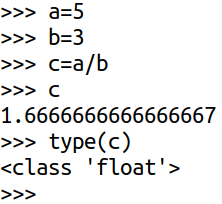
\includegraphics[scale=2.0]{pics/pembagian.png}
    \caption{Operator pembagian pada variabel berjenis \texttt{int} pada Python \texttt{3.x}}
    \label{fig:pembagian}
  \end{center}
\end{figure}


\begin{figure}
  \begin{center}
    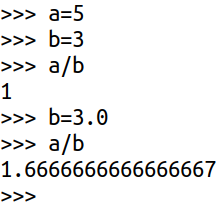
\includegraphics[scale=2.0]{pics/pembagian2.png}
    \caption{Operator pembagian pada variabel berjenis \texttt{int} pada Python \texttt{2.x}}
    \label{fig:pembagian2}
  \end{center}
\end{figure}

\subsection{Penugasan}
\tablename~\ref{tab:assignment} menunjukkan operator penugasan (\textit{assignment}) yang dimiliki Python.

\begin{table}[h]
\caption{Operator penugasan di Python}
\label{tab:assignment}
  \begin{center}
    \begin{tabular}{@{}ccc@{}}\toprule
    %\hline
    Operator & Contoh & Bentuk lain\\ \midrule
    = & x=7.5 & x=7.5\\
    += & x+=2 & x=x+2 \\
    -= & x-=2 & x=x-2\\
    *= & x*=3.1 & x=x*3.1\\
    /= & x/=5 & x=x/5\\
    \%= & x\%=2 & x=x\%2\\
    //= & x//=2 & x=x//2\\
    **= & x**=3 & x=x**3\\
       \bottomrule
    \end{tabular}
  \end{center}
\end{table}

\subsection{Perbandingan}
Operator perbandingan digunakan untuk menyatakan terjadinya kondisi tertentu. Perhatikan lagi sub bab \ref{sec:kondisi}. \tablename~\ref{tab:perbandingan} menunjukkan operator perbandingan yang dimiliki Python. 

\begin{table}[h]
\caption{Operator perbandingan di Python}
\label{tab:perbandingan}
  \begin{center}
    \begin{tabular}{@{}clc@{}}\toprule
    %\hline
    Operator & Fungsi  & Contoh\\ \midrule
    == & Kesamaan & a==b \\
    != & Ketidaksamaan & a!=b \\
    $<$ & Lebih kecil dari & $a<b$ \\
    $>$ & Lebih besar dari & $a>b$ \\
    $<=$ & Lebih kecil dari atau sama dengan & $a<=$ \\
    $>=$ & Lebih besar dari atau sama dengan & $a>=$ \\
       \bottomrule
    \end{tabular}
  \end{center}
\end{table}

\subsection{Logika}
\tablename~\ref{tab:logika} menunjukkan operator logika yang dimiliki Python.

\begin{table}[h]
\caption{Operator logika di Python}
\label{tab:logika}
  \begin{center}
    \begin{tabular}{@{}cll@{}}\toprule
    %\hline
    Operator & Deskripsi  & Contoh\\ \midrule
    \texttt{and} & \texttt{True} jika kedua pernyataan \texttt{True} & a==2 \texttt{and} b==3 \\
    \texttt{or} & \texttt{True} jika salah satu pernyataan \texttt{True} & a==2 \texttt{or} b==3 \\
    \multirow{2}{*}{\texttt{not}} & \multirow{2}{*}{Negasi} & \texttt{not}(a==2 \texttt{and} b==3) \\
     & & (tergantung nilai logika awal) \\
       \bottomrule
    \end{tabular}
  \end{center}
\end{table}

\subsection{Identitas}
\tablename~\ref{tab:identitas} menunjukkan operator identitas yang dimiliki Python.

\begin{table}[h]
\caption{Operator identitas di Python}
\label{tab:identitas}
  \begin{center}
    \begin{tabular}{@{}llc@{}}\toprule
    %\hline
    Operator & Fungsi  & Contoh\\ \midrule
    \multirow{2}{*}{\texttt{is}} & \texttt{True} jika kedua variabel merujuk  & \multirow{2}{*}{a \texttt{is} b} \\
    & pada obyek yang sama & \\
    \multirow{2}{*}{\texttt{is not}} & \texttt{True} jika kedua variabel merujuk & \multirow{2}{*}{a \texttt{is not} b} \\
    & pada obyek yang berbeda &\\
       \bottomrule
    \end{tabular}
  \end{center}
\end{table}

Perhatikan \figurename~\ref{fig:identitas}. Meski variabel \texttt{a} dab \texttt{b} bernilai sama (tentunya juga berjenis sama), tetapi mereka bukanlah obyek yang sama. Sehingga evaluasi menggunakan operator \texttt{is} menghasilkan nilai berbeda. Bandingkan dengan apa yang ditunjukkan \figurename~\ref{fig:identitas2}. Karena variabel \texttt{b} mengacu pada variabel \texttt{a}, maka evaluasi identitas \texttt{a} dan \texttt{b} menghasilkan nilai yang sama.

\begin{figure}
  \begin{center}
    \includegraphics[scale=2.0]{pics/identitas.png}
    \caption{Perbedaan respon evaluasi dua variabel berbeda dengan nilai yang sama}
    \label{fig:identitas}
  \end{center}
\end{figure}

\begin{figure}
  \begin{center}
    \includegraphics[scale=2.0]{pics/identitas2.png}
    \caption{Perbedaan respon evaluasi dua variabel identik dengan nilai yang sama}
    \label{fig:identitas2}
  \end{center}
\end{figure}

\subsection{Keanggotaan}
\tablename~\ref{tab:anggota} menunjukkan operator keanggotaan yang dimiliki Python.

\begin{table}
\caption{Operator keanggotaan di Python}
\label{tab:anggota}
  \begin{center}
    \begin{tabular}{@{}llc@{}}\toprule
    %\hline
    Operator & Fungsi  & Contoh\\ \midrule
    \multirow{2}{*}{\texttt{in}} & \texttt{True} jika nilai tertentu  & \multirow{2}{*}{a \texttt{in} b} \\
    & ada dalam obyek & \\
    \multirow{2}{*}{\texttt{not in}} & \texttt{True} jika nilai tertentu & \multirow{2}{*}{a \texttt{is not} b} \\
    & tidak ada dalam obyek &\\
       \bottomrule
    \end{tabular}
  \end{center}
\end{table}

Perhatikan \lstlistingname~\ref{lst:anggota}, di mana angka \texttt{7} yang di-\textit{assign} ke variabel \texttt{b} akan dicari di dalam list \texttt{a} yang berisi 20 angka yang diperoleh secara acak. Jika nilai \texttt{7} ada dalam \texttt{list a}, program akan mencetak teks \texttt{'Ada'}. Jika sebaliknya, program akan mencetak teks \texttt{'Tidak ada'}.

\lstinputlisting[language=python, numbers=left, numberstyle=\tiny, caption=Mendefinisikan fungsi sederhana, showstringspaces=false, label=lst:anggota]{script/anggota.py}

\chapter{Mendefinisikan fungsi dan menangani kesalahan}
\section{Mendefinisikan fungsi}
\subsection{Fungsi Umum}
Mendefinisikan fungsi di Python menggunakan kata kunci \texttt{def}, dilanjutkan dengan nama fungsi dan argumen (jika ada). Perhatikan \lstlistingname~\ref{lst:fungsi}. Fungsi \texttt{perkalian} menerima 2 argumen yang dapat dioperasikan secara aritmatika, dalam hal ini perkalian. Kita tidak perlu mendefinisikan jenis variabel \texttt{a} dan \texttt{b} sebagai argumen di fungsi tersebut. Jika variabel yang diberikan dapat digunakan di dalam fungsi, maka program akan berjalan sesuai yang diharapkan.

\lstinputlisting[language=python, numbers=left, numberstyle=\tiny, caption=Mendefinisikan fungsi sederhana, showstringspaces=false, label=lst:fungsi]{script/fungsi.py}

\subsection{\texttt{Lambda}}
\texttt{Lambda} adalah teknik yang tersedia di Python untuk mendefinisikan fungsi yang sederhana. Perhatikan \figurename~\ref{fig:lambda}. Di gambar tersebut ditunjukkan fungsi \texttt{lambda} yang melakukan perkalian terhadap dua bilangan.

\begin{figure}
  \begin{center}
    \includegraphics[scale=2.0]{pics/lambda.png}
    \caption{Contoh sederhana fungsi \texttt{lambda}}
    \label{fig:lambda}
  \end{center}
\end{figure}

\section{Menangani kesalahan (\textit{exception})}
\label{sec:error}
Coba perhatikan kembali \lstlistingname~\ref{lst:ulang} di sub bab \ref{sec:kondisi}. Kita dapat mengidentifikasi terjadinya kesalahan selain mengidentifikasi penyebabnya. Karena pada beberapa kasus, penyebab kesalahan sulit diidentifikasi di awal. Perhatikan \lstlistingname~\ref{lst:error}. Di \lstlistingname~\ref{lst:error}, jalannya program akan dihentikan ketika nilai \texttt{b} yang berperan sebagai pembagi bernilai \texttt{0}. 

\lstinputlisting[language=python, numbers=left, numberstyle=\tiny, caption=Menghentikan perulangan ketika didapati operasi yang tidak valid, showstringspaces=false, label=lst:error]{script/tangkapError.py}


\chapter{Membuat dan mengelola modul}
%script vs module: https://realpython.com/run-python-scripts/
\section{Pendahuluan}
\label{sec:awalmodul}
Modul dapat diartikan sebagai fungsi yang dapat dipanggil dari program Python apapun, selama lokasinya diketahui. Modul sangat berguna dalam menyederhanakan struktur aplikasi, sehingga setiap \textit{script} mengerjakan sedikit tugas utama yang saling terkait. Sedangkan tugas lain yang tidak terkait dipisahkan dalam \textit{script} yang bebeda di berkas yang berbeda. 

Perhatikan \lstlistingname~\ref{lst:faktorial} yang merupakan \textit{script} untuk menghitung nilai faktorial dari bilangan berjenis \texttt{int} yang dimasukkan. Faktorial, yang disimbolkan dengan \texttt{n!}, akan bernilai \texttt{n * n-1 * n-2 * $\ldots$ * 1}.

\lstinputlisting[language=python, numbers=left, numberstyle=\small, caption=Menghitung nilai faktorial, showstringspaces=false, label=lst:faktorial]{script/faktorial.py}

Jika perhitungan faktorial lebih dari satu kali, maka akan lebih efisien jika faktorial dibuat dalam fungsi tertentu yang dapat digunakan ulang tanpa menulis ulang. Perhatikan \lstlistingname~\ref{lst:faktorial2} di mana diperlukan dua kali pemanggilan terhadap fungsi \texttt{faktorial}. Dengan menerapkannya sebagai fungsi, kita tidak perlu menulis ulang fungsi \texttt{faktorial} (baris ke-1 s/d 8).

\pagebreak
\lstinputlisting[language=python, numbers=left, numberstyle=\small, caption=Menghitung nilai faktorial yang diterapkan sebagai fungsi, showstringspaces=false, label=lst:faktorial2]{script/faktorial2.py}

\section{Membuat modul}
Kita kembali ke kasus faktorial di sub bab \ref{sec:awalmodul}. Asumsikan jika ada beberapa \textit{script} yang membutuhkan fungsi \texttt{faktorial} tersebut. Maka, akan ada beberapa \textit{script} yang didalamnya terdefinisi fungsi \texttt{faktorial}. Pada kondisi inilah, modul memiliki peran penting. Perhatikan \lstlistingname~\ref{lst:faktorial3} yang penggunaannya memerlukan \textit{script} seperti \lstlistingname~\ref{lst:faktorialEks}.

\lstinputlisting[language=python, numbers=left, numberstyle=\small, caption=Fungsi faktorial sebagai modul, showstringspaces=false, label=lst:faktorial3]{script/faktorial3.py}

Maksud dari perintah di baris pertama \lstlistingname~\ref{lst:faktorialEks} adalah sebagai berikut.
\begin{itemize}
  \item \texttt{faktorial3} adalah nama file di mana modul faktorial didefinisikan (\texttt{faktorial3.py})
  \item \texttt{faktorail} adalah nama fungsi yang terdefinisi di modul faktorial
  \item \texttt{fk} adalah nama alias yang diberikan sebagai identitas fungsi \texttt{faktorial}. Fungsi dengan nama yang relatif panjang sering diberikan nama alias yang lebih singkat, terutama ketika fungsi tersebut sering digunakan
\end{itemize}

\lstinputlisting[language=python, numbers=left, numberstyle=\small, caption=\textit{Script} yang menggunakan modul \texttt{faktorial}, showstringspaces=false, label=lst:faktorialEks]{script/faktorialEks.py}

Pada kondisi lain, kita mungkin saja perlu melakukan pengujian terhadap modul yang kita bangun. Hal ini dapat disebabkan karena fungsinya kompleks sehingga selalu ada kemungkinan kesalahan dalam tahap pengembangannya. Maka, akan lebih mudah jika kita menyatukan \textit{script} yang bertugas untuk menguji dengan \textit{script} modul. Eksekusi terhadap \lstlistingname~\ref{lst:faktorial4} yang memanfaatkan modul seperti \lstlistingname~\ref{lst:faktorialEks2} akan menghasilkan luaran seperti pada \figurename~\ref{fig:modulUji}.

\lstinputlisting[language=python, numbers=left, numberstyle=\small, caption=Modul \texttt{faktorial} lengkap dengan fungsi ujinya, showstringspaces=false, label=lst:faktorial4]{script/faktorial4.py}

\lstinputlisting[language=python, numbers=left, numberstyle=\small, caption=\textit{Script} yang menggunakan modul \texttt{faktorial} yang di dalamnya ada fungsi uji, showstringspaces=false, label=lst:faktorialEks2]{script/faktorialEks2.py}

\begin{figure}
  \begin{center}
    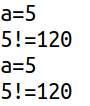
\includegraphics[scale=2.0]{pics/modulUji.png}
    \caption{Fungsi faktorial dipanggil dua kali}
    \label{fig:modulUji}
  \end{center}
\end{figure}

\figurename~\ref{fig:modulUji} menunjukkan bahwa fungsi \texttt{faktorial} dipanggil dua kali, masing-masing dari fungsi uji di luar modul dan fungsi uji di dalam modul. Untuk mengatasinya, perhatikan \lstlistingname~\ref{lst:faktorial5}. Dengan penambahan baris ke-8 di \lstlistingname~\ref{lst:faktorial5}, fungsi uji yang didefinisikan di modul tidak akan dieksekusi ketika modul tersebut sedang digunakan \textit{script} lain. \lstlistingname~\ref{lst:faktorial5} juga tampil lebih efisien dalam penulisan karena fungsi rekursif (pemanggilan fungsi itu sendiri) seperti ditunjukkan di baris ke-6.

\lstinputlisting[language=python, numbers=left, numberstyle=\small, caption=Modul \texttt{faktorial} lengkap dengan fungsi ujinya dan fungsi \texttt{main}, showstringspaces=false, label=lst:faktorial5]{script/faktorial5.py}

\section{Jejak pencarian}
Modul yang sebelumnya dibuat diletakkan di \textit{directory} yang sama dengan \textit{script} yang akan menggunakannya. Ketika lokasinya berbeda, maka modul tidak dapat digunakan. Agar dapat digunakan oleh \textit{script} di lokasi manapun, kita bisa meletakkan modul di lokasi standar dari modul. Dan untuk mengetahuinya, dapat dilakukan dengan menjalankan dua baris perintah berikut.

\texttt{>>> import sys}

\texttt{>>> sys.path}

Hasilnya adalah \texttt{list} yang berisi lokasi standar dari modul. Kita bisa meletakkan modul kita di lokasi tersebut. Sayangnya, lokasi tersebut umumnya memiliki kewenangan \texttt{root} untuk mengaksesnya sehingga kita tidak dapat melakukannya jika kita tidak memiliki hak akses \texttt{root}. Untuk kondisi ini, kita dapat menambahkan lokasi modul dengan \textit{directory user} kita. Karena dua perintah di atas menghasilkan \texttt{list}, kita bisa melakukan operasi \texttt{append} seperti contoh berikut.

\texttt{>>> import sys}

\texttt{>>> sys.path.append('/home/arya/Kuliah/PythonBasic/script/)}

Dengan demikian, semua \textit{script} Python yang ada di \textit{directory} tersebut dapat digunakan sebagai modul dari lokasi mana saja. Tetapi perlu diingat bahwa proses ini tidak permanen, hanya pada saat \textit{script} tersebut dieksekusi.

Terakhir, sebagai informasi, fungsi faktorial yang disajikan di sini hanya ilustrasi saja. Sejatinya, fungsi tersebut telah tersedia pada modul \texttt{math}.

\chapter{Interaksi berkas}
\section{Pendahuluan}
Lingkup interaksi di sini adalah interaksi dengan berkas teks (\texttt{ASCII}) untuk tujuan membaca, memformat ulang dalam bentuk penyajian di layar maupun disimpan kembali ke berkas teks. Selain teks, maka diperlukan proses tambahan untuk mengubahnya. Hal ini disebabkan karena umumnya data yang dianalisis dalam keilmuan data disimpan dalam bentuk teks dengan format csv (\textit{comma separated value}). Beberapa mungkin disimpan dalam aplikasi \textit{spreadsheet} seperti Microsoft Excel$\copyright$. 

Selain itu, kita mungkin saja terlibat dengan lebih dari satu berkas yang tersebar di \textit{sub directory}  yang berbeda. Atau bisa saja perlu menyusun ulang struktur \textit{directory} baru yang lebih mudah dipahami. Satu contoh kasus\footnote{\url{http://otmedia.lirmm.fr/LifeCLEF/PlantCLEF2017/}}, data yang berisi citra tumbuhan dari bagian yang berbeda seperti bunga, daun atau buah tidak tersusun berdasarkan bagian-bagian tersebut. Sementara kita memerlukan data tersebut tersusun berdasarkan bagian tumbuhan, bahkan mengikuti struktur \textit{family-genus-species}. Atau contoh lain\footnote{\url{https://www.unsw.adfa.edu.au/unsw-canberra-cyber/cybersecurity/ADFA-NB15-Datasets/bot\_iot.php}}, di mana dataset terpisah dalam berkas yang berbeda untuk kemudahan proses unduh. Sementara di masing-masing berkas terdapat data dari kelas-kelas yang berbeda. Untuk mengetahui proporsi data dari setiap kelas, kita perlu membaca semua potongan berkas yang tersedia.

\section{Berkas tunggal}
Sebagai bahan latihan, kita akan membaca dataset iris\footnote{\url{https://archive.ics.uci.edu/ml/machine-learning-databases/iris/iris.data}}. Pembacaan dilakukan baris per baris dan menampilkan isinnya. Dataset tersebut berisi informasi tentang dimensi bunga iris, yaitu \textit{sepal length}, \textit{sepal width}, \textit{petal length}, \textit{petal width} yang masing-masing dalam satuan \texttt{cm}. Kolom terakhir merupakan kelas dari 3 jenis bunga iris yang ada pada dataset tersebut, masing-masing Setosa, Versicolor dan Virginica. Data yang ditampilkan harus memiliki format 5 baris yang setiap barisnya adalah

\texttt{jenis bunga iris ke-i:}

\texttt{sepal length = $\ldots$ cm}

\texttt{sepal width = $\ldots$ cm}

\texttt{petal length = $\ldots$ cm}

\texttt{petal width = $\ldots$ cm}


Perhatikan \lstlistingname~\ref{lst:bacairis}. Program tersebut bertujuan untuk membaca data yang disimpan dalam bentuk tabular dan menampilkannya di layar dengan format baru. Simpan \lstlistingname~\ref{lst:bacairis} dalam berkas berekstensi \texttt{.py} lalu jalankan untuk melihat hasilnya dengan perintah \texttt{python nama\_file.py}.

\lstinputlisting[language=python, numbers=left, numberstyle=\small, caption=Membaca dataset iris dan menampilkan isinya dengan format tertentu, showstringspaces=false, label=lst:bacairis]{script/bacairis.py}

Berikut adalah penjelasan perintah pada \lstlistingname~\ref{lst:bacairis} berdasarkan urutan barisnya.
\begin{enumerate}
  \item Baris ke-1: membuat \texttt{pointer} ke berkas, yang dalam contoh ini adalah \texttt{iris.data} yang menjadi argumen pertama dari fungsi \texttt{open}. Sedangkan argumen keduanya adalah \texttt{'r'}, menunjukkan mode baca. Untuk mode tulis, gunakan argumen \texttt{'w'}.
  \item Baris ke-2: menyiapkan variabel \textit{dictionary} yang akan digunakan untuk menyimpan informasi kelas data berikut jumlahnya.
  \item Baris ke-3: menyiapkan variabel \texttt{int} yang akan digunakan untuk menyimpan informasi total data.
  \item Baris ke-4: memulai perulangan untuk membaca berkas per baris melalui perintah \texttt{a.readlines()}. Jika hanya diperlukan untuk membaca satu baris saja, gunakan perintah \texttt{a.readline()}. Baris yang berhasil dibaca akan disimpan dalam variabel \texttt{baris}.
  \item Baris ke-5 \& 18: penanganan kesalahan yang disebabkan oleh kondisi berkas yang baris terakhirnya kosong sehingga tidak dapat diolah seperti baris lain di atasnya.
  \item Baris ke-6: memisahkan baris yang dibaca berdasarkan pembatas (\textit{delimiter}) berupa karakter '\texttt{,}'. Hasilnya disimpan dalam \texttt{list} dengan nama \texttt{element}.
  \item Baris ke-7: membersihkan \texttt{element} terakhir dari karakter \escape{n}, dan menyimpannya dalan \texttt{list} dengan nama \texttt{kelas}. Nilai dari \texttt{kelas} yang akan digunakan disimpan di \texttt{kelas[0]}.
  \item Baris ke-8 s/d 11: blok kondisi yang ketika nilai kelas belum ada di variabel \texttt{jenis}, ia akan ditambahkan sebagai \texttt{key} dengan nilai \texttt{1}. Sedangkan jika sudah menjadi salah satu \texttt{key}, maka nilainya ditambah \texttt{1}.
  \item Baris ke-12 s/d 16: menampilkan isi dari baris yang sedang dibaca, yang sebelumnya telah dipisah-pisah ke layar. Sejatinya, perintah \texttt{print} menerima argumen \texttt{str}. Jika ada karakter/kata eksplisit akan ditampilkan bersama karakter/kata yang disimpan pada variabel, maka penulisannya perlu dibedakan, dan dihubungkan dengan operator \texttt{+}. Dari sini terlihat bahwa operator \texttt{+} tidak hanya dapat digunakan dalam operasi aritmatika. Khusus untuk variabel yang akan ditampilkan dengan perintah \texttt{print}, tetapi belum dalam bentuk \texttt{str} (seperti pada baris ke-12), maka perlu dilakukan transformasi. Perintah yang digunakan adalah \texttt{str}, sebagai target jenis variabel yang diperlukan. Jika pada kondisi tertentu, diperlukan untuk mengubah jenis variabel ke \texttt{int}, maka digunakan perintah yang sama dengan target jenis variabelnya, dalam hal ini \texttt{int}.
  \item Baris ke-17: mengakumulasi total data dari berkas yang dibaca.
  \item Baris ke-19: mendefinisikan perintah ketika baris yang dibaca tidak dapat diolah dengan perintah yang sama dengan baris lain.
  \item Baris ke-20: menghapus \texttt{pointer} ke berkas yang telah selesai digunakan.
  \item Baris ke-21: mencetak informasi
  \item Baris ke-22 \& 23: mencetak informasi statistik (jumlah data per kelas dan proporsinya dalam \%). Baris ke-22 digunakan untuk membuat perulangan berdasarkan jumlah kelas yang dalam contoh ini adalah jumlah elem dari variabel \texttt{jenis}. Sedangkan baris ke-23 digunakan untuk mencetak informasi berikut:
  \begin{itemize}
     \item nama kelas yang direpresentasikan melalui variabel \texttt{i}.
     \item jumlah data untuk kelas tertentu yang direpresentasikan melalui variabel \texttt{jenis[i]}. Karena jenisnya \texttt{int}, maka perlu diubah ke \texttt{str}.
     \item proporsi jumlah data, dilakukan dengan cara melakukan operasi pembagian jumlah data per kelas terhadap total data. Hasilnya ditampilkan dengan format dua angka desimal (\texttt{:4.2f}).
   \end{itemize} 
   Hasil dari menampilkan informasi statistik tersebut ditampilkan di \figurename~\ref{fig:iristat}.
\end{enumerate}

\begin{figure}
  \begin{center}
    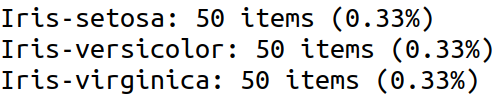
\includegraphics[scale=2]{pics/iristat.png}
    \caption{Informasi statistik dataset iris}
    \label{fig:iristat}
  \end{center}
\end{figure}

\section{Berkas jamak}
Selanjutnya, sebagai latihan kedua, dataset yang akan digunakan adalah dataset tentang keamanan siber\footnote{\url{https://www.unsw.adfa.edu.au/unsw-canberra-cyber/cybersecurity/ADFA-NB15-Datasets/bot\_iot.php}}. Untuk seluruh dataset, terdapat 74 berkas yang berbeda. Tetapi, berkas pertamanya kosong sehingga akan diabakan dalam pembacaan. Perhatikan \lstlistingname~\ref{lst:catexplore}.

\lstinputlisting[language=python, numbers=left, numberstyle=\small, caption=Menghitung total data untuk setiap kelas, showstringspaces=false, label=lst:catexplore]{script/categoryExplore.py}

\section{Modifikasi dataset}
Yang dimaksud dengan modifikasi di sini adalah memilih bagian yang menarik untuk dianalisis. Sebagai contoh, salah satu dataset tentang keamanan siber\footnote{https://github.com/aawaskita/Cyber-Security-dataset/} memiliki fitur yang dapat dibagi menjadi beberapa kelompok. \lstlistingname~\ref{lst:featbased} mengilustrasikan bagaimana memisahkan data berdasarkan kelompok fitur tersebut. Kita bisa saja melakukan kajian tentang efektivitas penggunaan kelompok fitur yang berbeda terhadap akurasi suatu \textit{classifier}. Untuk dapat diklasifikasi, kolom kelas tetap disimpan di dataset untuk kelompok fitur berbeda.

\lstinputlisting[language=python, numbers=left, numberstyle=\small, caption=Memisahkan dataset ke dalam kelompok fitur yang berbeda, showstringspaces=false, label=lst:featbased]{script/featureBasedAttack.py}

Penjelasan baris-baris perintah dari \lstlistingname~\ref{featbased} adalah sebagai berikut.
\begin{enumerate}
  \item Baris ke-1 s/d 6: membuat \texttt{pointer} ke berkas sumber (baris ke-1) maupun berkas target (baris ke-2 s/d 6). Kelompok fitur yang dimaksud masing-masing adalah diwakili oleh \texttt{pointer} yang dibuat di baris ke-2 s/d 6.
  \item Baris ke-7 s/d 12: membuat penanda kolom di mana kelompok fitur diletakkan di berkas sumber. Sebagai contoh, fitur \textit{basic} disimpan di kolom 6 s/d 18. Maka, untuk mengambil data dari kelompok fitur \textit{basic}, gunakan data yang disimpan kolom 6 s/d 18.
  \item Baris ke-13: memulai perulangan untuk membaca berkas baris per baris.
  \item Baris ke-14: memisahkan baris yang dibaca berdasarkan pembatas (\textit{delimiter}) berupa karakter '\texttt{,}'. Hasilnya disimpan dalam \texttt{list} dengan nama \texttt{element}.
  \item Baris ke-15: menyimpan data kelas yang disimpan di lokasi terkahir dari \texttt{element}.
  \item Baris ke-16 s/d 21: mengambil data dari 5 kolom pertama sebagai data yang harus ada di setiap kelompk fitur.
  \item Baris ke-23 s/d 25: mengambil data untuk kelompok fitur \textit{basic} dan diakhiri dengan menyimpan kelas data di kolom terakhir. Fungsi yang sama berlaku untuk
  \begin{itemize}
     \item baris ke-27 s/d 29 (untuk kelompok fitur \textit{content}),
     \item baris ke-31 s/d 33 (untuk kelompok fitur \textit{time}),
     \item baris ke-35 s/d 37 (untuk kelompok fitur \textit{general})
     \item serta baris ke-39 s/d 41 (untuk kelompok fitur \textit{connection}).
   \end{itemize}
   \item Baris ke-43 s/d 48: menghapus \texttt{pointer} ke berkas yang telah digunakan.
\end{enumerate} 

\section{Latihan}
\begin{enumerate}
  \item Modifikasi \lstlistingname~\ref{lst:bacairis} agar dapat dijalankan tanpa perlu pengetahuan tentang jumlah kolom
  \item Dataset\footnote{\url{https://www.unsw.adfa.edu.au/unsw-canberra-cyber/cybersecurity/ADFA-NB15-Datasets/bot\_iot.php}} menyediakan informasi sub kelas. Sebagai contoh, kelas \texttt{UDP} memiliki sub kelas \texttt{Dos} dan \texttt{DDoS}. Sementara \lstlistingname~\ref{lst:catexplore} hanya menampilkan informasi jumlah data per kelas. Karena itu, modifikasi \lstlistingname~\ref{lst:catexplore} agar dapat secara otomatis menghitung jumlah data per kelas sekaligus per sub kelas dan menampilkannya di layar.
  \item Berdasarkan pengetahuan yang diperoleh dari \lstlistingname~\ref{lst:featbased}, bangun program sejenis yang mampu memisahkan data pada Latihan kedua yang hanya berisi data-data dari dua kelas terbesar. Pengetahuan tentang dua kelas terbesar diperoleh dari Latihan kedua.
\end{enumerate}

\chapter{Interaksi Basisdata}
\section{MySQL}
%create user: create user 'arya'@'localhost' identified by '123456';
%create database: create database iris;
%grant user: grant all on 'iris.* to 'arya'@'localhost';
%flush privileges;
%create table irisdata (sepallength real(2,1), sepalwidth real(2,1), petallength real(2,1), petalwidth real(2,1), kelas varachr(15));
Modifikasi \lstlistingname~\ref{lst:bacairis} sehingga menjadi seperti \lstlistingname~\ref{lst:insertiris}. Hasil ekseksinya ditunjukkan \figurename~\ref{fig:insertmysql}.
 
\lstinputlisting[language=python, numbers=left, numberstyle=\small, caption=Membaca dataset iris dan menyimpannya di MySQL, showstringspaces=false, label=lst:insertiris]{script/insertiris.py} 

\begin{figure}
  \begin{center}
    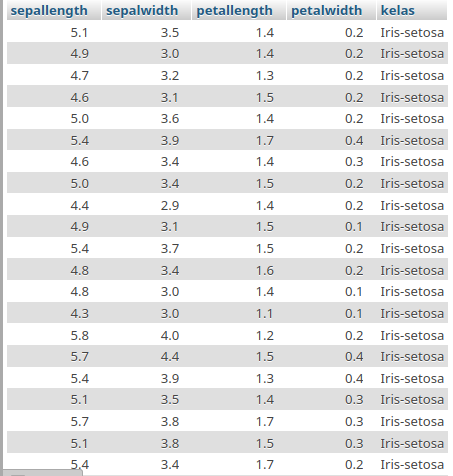
\includegraphics[scale=2.0]{pics/insertmysql.png}
    \caption{Hasil dari proses memasukkan data ke server MySQL}
    \label{fig:insertmysql}
  \end{center}
\end{figure}
\section{PostgreSQL}
Modifikasi \lstlistingname~\ref{lst:insertiris} sehingga menjadi seperti \lstlistingname~\ref{lst:insertirispg}. Hasil ekseksinya ditunjukkan \figurename~\ref{fig:insertpgsql}.

\lstinputlisting[language=python, numbers=left, numberstyle=\small, caption=Membaca dataset iris dan menyimpannya di pgSQL, showstringspaces=false, label=lst:insertirispg]{script/insertirispg.py}

\begin{figure}
  \begin{center}
    \includegraphics[scale=2.0]{pics/insertpgsql.png}
    \caption{Hasil dari proses memasukkan data ke server pgSQL}
    \label{fig:insertpgsql}
  \end{center}
\end{figure}

%https://computingforgeeks.com/installing-postgresql-database-server-on-ubuntu/
%https://linuxhint.com/postgresql_installation_guide_ubuntu_20-04/
%https://www.howtoforge.com/tutorial/ubuntu-postgresql-installation/
\section{MongoDB}
MongoDB adalah salah satu basisdata non-relasional yang menyimpan data berbasis dokumen. Bukan dokumen seperti berkas yang digunakan pengolah teks seperti Microsoft Word$\copyright$, tetapi JSON (\textit{JavaScript Object Notation}) seperti dilustrasikan \figurename~\ref{fig:jsonmongo}\footnote{\url{https://www.mongodb.com/blog/post/getting-started-with-python-and-mongodb}}.

\begin{figure}
  \begin{center}
    \includegraphics[scale=.75]{pics/JSONExamplePythonMongoDB.png}
    \caption{Ilustrasi penyimpanan data berbasis dokumen oleh MongoDB}
    \label{fig:jsonmongo}
  \end{center}
\end{figure}

Sedangkan \tablename~\ref{tab:relasimongo} menunjukkan perbandingan konsep pada basisdata relasional terhadap basisdata non-relasional seperti MongoDB\footnote{\url{https://www.mongodb.com/blog/post/getting-started-with-python-and-mongodb}}.

\begin{table}[h]
\caption{Komparasi konsep basisdata relasional vs. non-relasional}
\label{tab:relasimongo}
  \begin{center}
    \begin{tabular}{@{}cc@{}}\toprule
    %\hline
    Relasional & Non-relasional\\ \midrule
  \textit{Database} & \textit{Database} \\ 
  \textit{Table} & \textit{Collection} \\
  \textit{Rows} & \textit{Documents}\\
  \textit{Index} & \textit{Index}\\
       \bottomrule
    \end{tabular}
  \end{center}
\end{table}

Sebagai bahan latihan, kita akan menggunakan dataset yang digunakan dalam artikel \cite{peerreview}\footnote{\url{https://github.com/allenai/PeerRead}}. Perhatikan \lstlistingname~\ref{lst:readjson} yang bertujuan untuk mengeksplorasi struktur berkas json secara rekursif. Dari \lstlistingname~\ref{lst:readjson} kita dapat mengambil pasangan \textit{key}-\textit{value} dari struktur berkas json.

\lstinputlisting[language=python, numbers=left, numberstyle=\small, caption=Mengeksplorasi struktur berkas json, showstringspaces=false, label=lst:readjson]{script/readjson.py}

Setelah berhasil melakukan pembacaan berkas json, sekarang saatnya mencoba memasukkan data berkas json ke MongoDB. Perhatikan \lstlistingname~\ref{lst:savejson}.

\lstinputlisting[language=python, numbers=left, numberstyle=\small, caption=Menyimpan berkas json ke MongoDB, showstringspaces=false, label=lst:savejson]{script/savemongo.py}

 


%https://www.geeksforgeeks.org/how-to-import-json-file-in-mongodb-using-python/
%https://www.w3schools.com/python/python_mongodb_getstarted.asp
%https://www.programiz.com/python-programming/json
%https://www.geeksforgeeks.org/python-mongodb-query/?ref=rp


%\chapter{Sub Modul Pustaka \texttt{Scikit-Image}}

\bibliographystyle{apalike}
\bibliography{reference}
\end{document}
